\documentclass[palatino]{epflnotes}

\title{Hydrodynamics}
\author{Guillermo Julián}
\date{16/17 - Spring semester}

% Additional packages
\usepackage{siunitx}
% --------------------

\begin{document}
\frontmatter
\pagestyle{plain}
\maketitle

\tableofcontents
\mainmatter
% Content

\chapter{Introduction}

\section{Some definitions on physics}

Some important definitions. Let $p$ be the pressure, $F$ force, $A$ areas. Then $p = \frac{F}{A}$. If we have dynamic pressure (exerted by a fluid moving) then $p = \frac{1}{2}ρu^2$ and we can see the force exerted by a liquid on a surface as \[ \vF = \int_S \frac{1}{2} ρ u_\perp^2 \dif S \] where $u_\perp$ is the component of $u$ perpendicular to $S$.

The buoyancy of Archimedes law is given by \[ F = (ρ_f - ρ_b) g V \] with $V$ the volume of the body, $ρ_f$ the densitiy of the fluid and $ρ_b$ the density of the body.

Regarding viscosity, the dynamic viscosity μ is a measure of internal resistance, measured in $\si{\pascal\second} \equiv \si{\newton\second\per\metre\squared}$ while the kinematic visocosity is given by $ν = \sfrac{μ}{ρ}$ and measure in $\si{\metre\squared\per\second}$, where $ρ$ is the density of the fluid measured in $\si{\kilogram\per\cubic\metre}$.

For example, the viscosity of air is $\SI{18.1e-6}{\pascal\second}$ and that of water is $\SI{8.9e-4}{\pascal\second}$. More or less same values for dynamic viscosity for air, for water $\SI{8.9e-7}{\metre\squared\per\second}$.

One can calculate the stress on the boundary with no-slip conditions as \[ τ(y) = μ\dpd{u}{y}\] with $u$ the flow velocity along the boundary, $y$ the height abouve the boundary and $μ$ the dynamic viscosity of the flow. We can get the force exerted because $f = \int_{S} τ\dif S $.

The volumetric flow rate is defined as \[ Q = \iint_A \vU · \vn_A \dif A \] where $A$ is a surface and $\vn_A$ its normal vector.

We can also use the Bernoulli equation that says that \[ P_0 + \frac{1}{ρ}v^2 +ρ  gh = C\] is constant, with $P_0$ the pressure, ρ the density, $v$ the velocity and $h$ the height of a fluid. Only valid for steady flow, however.

\section{Fundamental laws of hydrodynamics}

\subsection{Transport theorem and conservation of mass}

The transport theorem models the change of a certain quantity enclosed in a volume $Ω$. That change responds to changes in the quantity to measure and in the shape of Ω.

\begin{theorem}[Transport\IS theorem] Let $Ω(t) ∈ ℝ^3$ be a volume shape, with its shape change modeled by the velocity field $\appl{\vu}{ℝ^3 × ℝ}{ℝ}$ and $\appl{b}{ℝ^3×ℝ}{ℝ}$ the quantity being modeled. Then, the change over time of the total flux can be expressed as \( \od{}{t} \int_{Ω(t)} b(\vx, t) \dif V_t = \int_{Ω(t)} \dpd{b}{t} \dif V_t + \int_{∂Ω(t)} (\vu · \vn) b(\vx, t) \dif A_t \label{eq:TransportTheorem} \) where $\vn$ is the normal to $Ω(t)$, and $V_t, A_t$ are the volume and are elements of $Ω(t)$.
\end{theorem}

Basically, this theorem says that the change is accounted for by the change of the quantity itself plus the change of the flux exiting or entering the volume.

There are several expressions for conservation of mass based on \eqref{eq:TransportTheorem}:
\begin{align*}
\od{}{t}\iiint_Ω ρ \dif V + \iint_{∂Ω} ρ\vu \dif A &\qquad \text{Integral conservation form}\\
\frac{\Dif}{\Dif t} \iiint_V ρ \dif V = 0 &\qquad \text{Integral nonconservation form}\\
\dpd{ρ}{t} + \dv (ρ \vu) = 0 &\qquad \text{Differential conservation} \\
\frac{\Dif ρ}{\Dif t} + ρ \dv \vu = 0 &\qquad \text{Differential nonconservation}
\end{align*} where $ρ$ is the density of the fluid.

For an incompressible flow, we have $ρ$ constant and then we have $\dv \vu = 0$, which is usually called the \concept{Continuity\IS equation}.

\subsection{Stress modeling and momentum conservation}

Then some equation \[ ρ \od{b}{t} = Q + \dv A\] where $A$ are volume sources and $A$ surface fluxes.

For the surface forces, we can use a theorem due to Cauchy that shows that the surface force can be represented by a stress tensor\footnote{Also known in this context as a $3 × 3$ matrix.}, so the force is $\vt = σ \vn$.

We will divide the stresses in the fluid in two parts: one static, existing even in the abscene of motion (that is, pressure); and another one related to motion.

Pressure exerts a force normal to the surface, that is, $\vf(x) = -p(x) \vn(x)$ and the stress tensor is $σ = -p(x) I $ with $I$ the identity matrix.

For stresses in a moving fluid, we add forces tangential to the surface that are represented by a second part of the stress tensor, $τ(\vx)$, that is called the viscous stress tensor.

The viscous stress tensor has two group of components, $τ_{xx}, τ_{yy}, τ_{zz}$ which are the stretching terms; and the other ones (symmetric) which are the shear terms. Thus conservation of momentum is given by \[ ρ \frac{\Dif \vu}{\Dif t} = \dv σ + ρ \vf \]


\subsection{Navier-Stokes for incompressible fluids}

In our incompressible flow, we have that the viscous tensor is the symmetric part of the velocity so that $D = \frac{\trans{∇u} + ∇u}{2}$ and $ σ = - pI + 2μD$ and thus putting everything together the results is \begin{align*}
ρ \frac{\Dif \vu}{\Dif t} &= - ∇p + μΔ\vu + ρ \vf \\
\dv \vu &= 0
\end{align*}

In order to solve these equations, boundary conditions will be set at time $t = 0$ (initial conditions); and also at the interfaces.

For example, for liquid/solid interfaces, we will use either no-slip boundary conditions ($\vu_\text{liquid} = \vu_\text{solid}$ at the interface) or non-penetration ($\vu_\text{liquid} · \vn = \vu_\text{solid} · \vn$).

For liquid/liquid interfaces, we will have continuity of velocity $\vu_1 = \vu_2$, free-slip conditions ($\vu_{1} · \vn = \vu_{2} · \vn = \vv_\text{interface}$) or continuity of stress ($σ_1 · \vn = σ_2 · \vn$).

Finally, for liquid/gas interfaces (free surfaces), we have either no-slip or no-stress ($σ·\vn = 0$).

We will also non-dimensional equation in which we use gauges to measure the quantities of interest for the problem.

\section{Dimensional analysis}

We can reduce models to study only the effect of the most important parameters. One can choose a reference scale using the relevant parameters. Then, we replace in the corresponding equations, apply dominant balance principle (avoid removing magnitudes too early) and then remove the things that are unimportant.

\chapter{Stokes flow}

In this chapter we will consider Stokes flow, also called creeping flow. This is a type of flow with small Reynolds number ($\rey \ll 1$) and therefore is a type of flow where the advective inertial forces are small compared with viscous forces. The Stokes equations for an incompressible Newtonian fluid are given by \begin{align*}
μ Δu - ∇p + \vf &= \vec{0} \\
\dv \vu &= 0
\end{align*}


First, we will need to introduce the streamfunction, which greatly simplifies the study of this flow.

\section{Streamfunction}

\begin{defn}[Streamfunction] \label{def:Streamfunction} For a given 2-dimensional incompressible flow, the streamfunction $ψ(x,y,t)$ is defined as the volume flux through a curve from $A_0$ (a reference point) to the point $(x,y)$. This gives the following expressions for velocity $\vU = (u, v, 0)$ of the flow (in cartesian coordinates):
\( u = \dpd{ψ}{y} \qquad v = - \dpd{ψ}{x} \label{eq:StreamfunctionCartesian}\)
\end{defn}

The interesting thing about the streamfunction is that by its definition it can only applied to incompressible fluids. Indeed, if we calculate the divergence of the flow we have \[ \dv \vU = \dpd{u}{x} + \dpd{v}{y} = \mder{ψ}{2}{x}{}{y}{} -\mder{ψ}{2}{y}{}{x}{} = 0 \]

If we change to cylindrical coordinates with axisymmetry (remember that streamfunction model 2D flows), the equations change to \( \label{eq:StreamfunctionCylindricalAxisym} u = \frac{1}{r} \dpd{ψ}{r} \qquad v = - \frac{1}{r} \dpd{ψ}{z} \) and one can check that we still have conservation of mass.

\subsection{Relation to vorticity}

Remember that the vorticity of a flow is defined as $\vec{ω} = \rot \vU$. If we use the streamfunction formulation, we end up with the following short expression:
\[ \vec{ω} = - Δψ \ve_z\] which is incredibly convenient. Using this expressions in Navier-Stokes equations we would end up with advection-diffusion forms:
\[ \dpd{ω}{t} + u \dpd{ω}{x} + v \dpd{ω}{y} = ν Δω \]

\section{Stokes equation}

In order to derive the Stokes equation, we start off from Newton incompressible flow equations:
\[ ρ \frac{\Dif \vU}{\Dif t} = - ∇ p + μ Δ \vU + ρ\vf \]

Assuming no external forces ($\vf \equiv 0$) and steady flow, we have the following simplification:
\( \begin{aligned}
ηΔ\vU &= ∇p \\
\dv \vU &= 0
\end{aligned} \label{eq:StokesFlow} \)

We can derive that to other formulations:
\begin{gather*}
Δp = 0 \\
Δω = 0
\end{gather*}

The last one gives rise to the biharmonic equation: \[ ∇^4 ψ = Δ(Δψ) = 0 \] which is a fully determined equation once we put in boundary conditions.

An interesting fact from the linearity of the equations is that the flow is reversible: if we change the sign we have still a solution.

Additionally, the unique solution of the Stokes equations with suitable boundary conditions is the divergence free flow field that minimizes viscous dissipation, which is given by \[ φ = 2 μ \int e_{ij} e_{ij} \dif V \]

\subsection{Flow along a sphere}

We are going to study the flow along a sphere of radius $a$, in order to see why the falling. In this case, the Stokes streamfunction in spherical coordinates is given by
\( \label{eq:FlowSphereStokes}\begin{aligned}
U_r(r,θ) &= \frac{1}{r^2 \sin θ} \dpd{ψ}{θ} \\
U_θ(r,θ) &= -\frac{1}{r \sin θ} \dpd{ψ}{r}
\end{aligned} \)

We can also look at the rotational in spherical coordinates, which is \[ \vec{ω} = \rot \vU = \frac{1}{r} \left( \dpd{rU_θ}{r} - \dpd{U_r}{θ}\right)\ve_φ = - \frac{1}{r\sin θ} \left(\dpd[2]{ψ}{r} + \frac{1}{r^2} \dpd[2]{ψ}{θ} - \frac{\cot θ}{r^2} \dpd{ψ}{θ}\right) \ve_ψ \] and therefore we have the final equation of the bilaplacian as \( Δ^2_s ψ ≝ \left(\dpd[2]{}{r} + \frac{1}{r^2} \dpd[2]{}{θ} - \frac{\cot θ}{r^2} \dpd{}{θ}\right)^2 ψ = 0 \label{eq:BilaplacianSphereFlow} \)

For the boundary conditions, in the frame of the sphere we have no-slip and thus $u_r(a, θ) = u_θ(a, θ) = 0$. By plugging this into the expression of the flow from \eqref{eq:FlowSphereStokes}, we find the following restriction on the streamfunction: \[ ψ(a, θ) = \dpd{ψ}{r}(a, θ) = 0 \]

We also need far-field boundary conditions. When $r \to ∞$, we want $\vU(r, θ) \to U_∞ \ve_z$, so that we need \[ U_r \sim U_∞ \cos θ \qquad U_θ \sim -U_∞ \sin θ \quad\text{when } r \to ∞\]

Plugging that in \eqref{eq:FlowSphereStokes}, we have that \begin{align*}
\frac{1}{r^2 \sinθ} \dpd{ψ}{θ} &\convs[][r][∞] U_∞ \cos θ \\
\dpd{ψ}{θ} &\convs[][r][∞] U_∞ r^2 \cos θ \sin θ \\
ψ &\convs[][r][∞] \frac{U_∞r^2 \sin^2 θ}{2}
\end{align*} and doing that with $U_θ$ yields the same result. We are using, though, a very informal definition of convergence of functions.

We are going to suppose that the solution is of the form $ψ = f(r) \sin^2 θ$. We can compute the derivatives of this thing:
\begin{align*}
\dpd{ψ}{θ} &=  2 f(r) \sin θ \cos θ \\
\dpd[2]{ψ}{θ} &= 2 f(r) (\cos^2 θ - \sin^2 θ)
\end{align*}

Putting that in the equation of the bilaplacian \eqref{eq:BilaplacianSphereFlow}, we will have that \[Δ_s ψ = f'' \sin^2 θ + \frac{2f}{r^2} (\cos^2 θ  - \sin^2 θ) - \frac{\cos θ}{r^2 \sin θ} 2f(r) \sin θ \cos θ  \]

Computing the laplacian again we end up with \[ Δ_s^2 ψ = \left(\dod[2]{}{r} - \frac{2}{r^2}\right)^2 f \]

\section{Hele-Shaw flow}

\begin{figure}[hbtp]
\centering
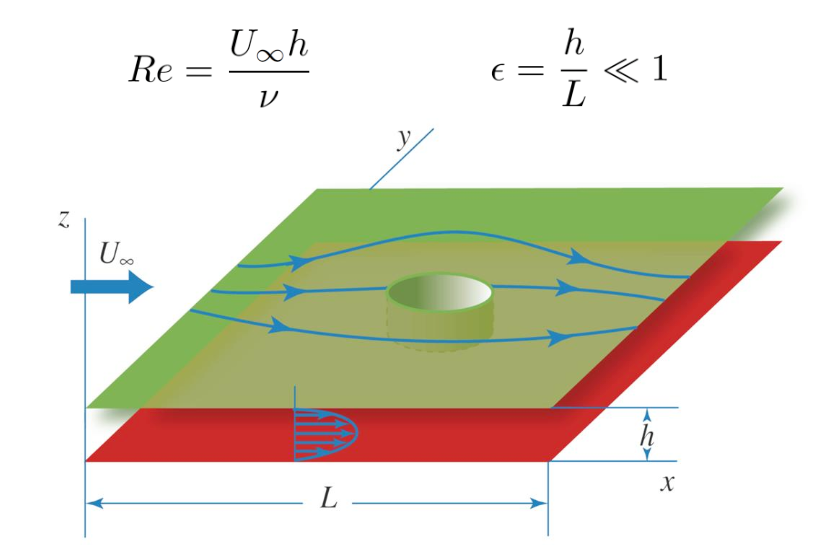
\includegraphics[width=0.8\textwidth]{img/HeleShaw.png}
\caption{Hele-Shaw flow in a thin cell.}
\label{fig:HeleShaw}
\end{figure}

One example of Stokes flow is the Hele-Shaw cell, which is the flow between two plates in a narrow gap. Even though it is a viscous-dominated flow, it will behave like potential flow which is traditionally for high reynolds numbers.

In this case we will use different length gauges for the $x$ and $y$ directions (in-plane) and for the $z$ direction (perpendicular to the plane). That induces different scalings on the velocities and that will change things in the continuity equation:
\begin{align*}
\dpd{x}{u} + \dpd{y}{v} + \dpd{z}{w} &= 0 \\
\frac{U_∞}{L} \dpd{\tilde{u}}{\tilde{x}} + \frac{U_∞}{L} \dpd{\tilde{v}}{\tilde{y}} + \frac{W}{h} \dpd{\tilde{w}}{\tilde{z}} &= 0 \\
\dpd{\tilde{u}}{\tilde{x}} + \dpd{\tilde{v}}{\tilde{y}} + \frac{WL}{hU_∞} \dpd{\tilde{w}}{\tilde{z}} &= 0
\end{align*}

Here, for the selection of the gauge $W$ we still cannot neglect anything so we will apply \concept{Dominant balance transport} or principle of least degeneracy: we want to keep things as open as possible. So, we will choose $W$ such that all the derivatives in the continuity equation have the same magnitude: \[ W = \frac{U_∞h}{L} \]

Now we go to the Navier-Stokes equations getting rid of the time derivatives (flow is steady)
\begin{align*}
u \dpd{u}{z}  + v \dpd{u}{y} + w \dpd{u}{z} &= - \frac{1}{ρ} \dpd{p}{x} + ν \left(\dpd[2]{u}{x} + \dpd[2]{u}{y} + \dpd[2]{u}{z}\right) \\
\frac{U_∞^2}{L} u \dpd{\tilde{u}}{\tilde{z}}  + \frac{U_∞^2}{L} v \dpd{\tilde{u}}{\tilde{y}} + \frac{WU_∞}{h} w \dpd{\tilde{u}}{\tilde{z}} &= - \frac{U_∞^2}{L}\frac{1}{ρ} \dpd{p}{x} + \frac{P}{ρL} ν \left(\frac{U_∞}{L^2} \dpd[2]{\tilde{u}}{\tilde{x}} + \frac{U_∞}{L^2} \dpd[2]{\tilde{u}}{\tilde{y}} + \frac{U_∞}{h^2} \dpd[2]{\tilde{u}}{\tilde{z}}\right)
\end{align*}

In the Laplacian, the term with $\frac{1}{h^2}$ is going to dominate so we can neglect the two other terms of that Laplacian, and that gives us the pressure gauge \[ P = \frac{νU_∞ ρL}{h^2} \] which in turn creates an effective Reynolds number which is considerably lower than the one we would measure with more naive gauges: \[ \rey = \frac{U_∞h^2}{νL} \]

We can do the same for the velocity in the Z direction:
\begin{align*}
u \dpd{w}{z}  + v \dpd{w}{y} + w \dpd{w}{z} &= - \frac{1}{ρ} \dpd{p}{z} + ν \left(\dpd[2]{w}{x} + \dpd[2]{w}{y} + \dpd[2]{w}{z}\right) \\
\frac{U_∞^2h}{L} \left(u \dpd{\tilde{w}}{\tilde{z}}  + v \dpd{\tilde{w}}{\tilde{y}} + w \dpd{\tilde{w}}{\tilde{z}}\right)
	&= - \frac{P}{ρh} \dpd{p}{z} + \frac{νU_∞}{Lh} \left(\cancelto{0}{\dpd[2]{\tilde{w}}{\tilde{x}} + \dpd[2]{\tilde{w}}{\tilde{y}}} + \dpd[2]{\tilde{w}}{\tilde{z}}\right) \\
\rey \frac{h^2}{L^2} \left(u \dpd{\tilde{w}}{\tilde{z}}  + v \dpd{\tilde{w}}{\tilde{y}} + w \dpd{\tilde{w}}{\tilde{z}}\right)
	&= - \frac{L^2}{h^2} \dpd{p}{z} + \dpd[2]{\tilde{w}}{\tilde{z}}
\end{align*}
neglecting as previously the $x, y$ derivatives of the laplacian and dividing in the last equation by $\frac{νU_∞}{Lh}$. There, the term that is going to dominate is the pressure one, so we can neglect the others and we have that \[ \dpd{p}{z} = 0\]

Note that had we started in the reverse order, we would have ended with a pressure gauge that would lead to the condition $ν ∂^2_z u = 0$, which gives a linear solution to $u$ that is not going to satisfy the boundary conditions.

Following this line of reasoning we end up with the fundamental equations of the Hele-Shaw flow:
\begin{align*}
\dpd{u}{x} + \dpd{v}{y} + \dpd{w}{z} &= 0 \\
μ \dpd[2]{u}{z} &= \dpd{p}{x} \\
μ \dpd[2]{v}{z} &= \dpd{p}{y} \\
\dpd{p}{z} &= 0
\end{align*}

That gives the equations that are on the slide and the solutions on the slide too. The solution is then potential flow. Furthermore, if we inject the solutions in the continuity equation we get
\begin{align*}
- \frac{1}{2μ}\left(\dpd[2]{p}{x} + \dpd[2]{p}{y}\right) z(z - h) &= - \dpd{w}{z} \\
\frac{z^3}{3} -  \frac{z^2h}{2} + C &= w
\end{align*}

To satisfy boundary conditions, we say $w(0) = 0$ so that $C = 0$, but then $w(h) ≠ 0$. The only option is then having \[ - \frac{1}{2μ}\underbracket{\left(\dpd[2]{p}{x} + \dpd[2]{p}{y}\right)}_{Δ_{\parallel} p} = 0 \implies Δ_\parallel p = 0 \] which in turn gives zero vorticity.

Of course all of this is extremely shady and non-mathematical. A validation is something. Intertial terms next slide this is weird. We can see that the flow in a rectangular duct is a good approximation of this. Then we can compute the flow rate which simplifies to \[ Q = \frac{h^3}{12μ} \dpd{p}{x} \] which is compatible with the inexact solution when $h \ll w$ (take $Q$ as the flux over width $w$).

\section{Lubrication}

\begin{wrapfigure}[6]{R}{0.4\textwidth}
\centering
\vspace{-15pt}
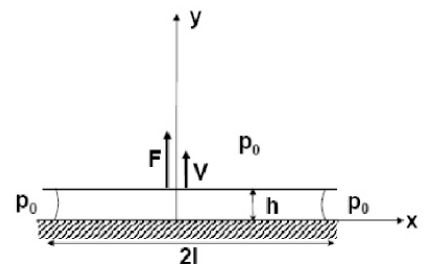
\includegraphics[width = 0.4\textwidth]{img/DuctTape.png}
\caption{Duct tape 2-dimensional flow}
\label{fig:DuctTape}
\end{wrapfigure}

One interesting situation is to study how duct tape glues (\fref{fig:DuctTape}). As usual, we start off from the 2-dimensional stokes equations
\begin{align*}
\dpd{u}{x} + \dpd{v}{y} &= 0 \\
\dpd{p}{x} - μ \left( \dpd[2]{u}{x} + \dpd[2]{u}{y} \right) &= 0 \\
\dpd{p}{y} - μ \left( \dpd[2]{v}{x} + \dpd[2]{v}{y} \right) &= 0
\end{align*}

First, we perform a dimensional analysis with the following scales:
\begin{align*}
x &= l\tilde{x} & y = h \tilde{y} \\
u &= U \tilde{u} & v = V \tilde{v} \\
p &= P \tilde{p}
\end{align*}

Introducing them in the continuity equation we get
\[ \dpd{u}{x} + \dpd{v}{y} = 0 \implies \frac{U}{l} \dpd{\tilde{u}}{\tilde{x}} + \frac{V}{h} \dpd{\tilde{v}}{\tilde{y}} = 0\]

Following the dominant balance principle, we would want to keep both terms so we set the gauge for $V$ as $V = \frac{Uh}{l}$ with $V \ll U$ as $h \ll l$, and therefore we end up with continuity equation on the nondimensional variables \[ \dpd{\tilde{u}}{\tilde{x}} + \dpd{\tilde{v}}{\tilde{y}} = 0 \]

In the momentum equation along $x$ we get
\[ \dpd{p}{y} - μ \left( \dpd[2]{v}{x} + \dpd[2]{v}{y} \right) = 0 \implies \frac{P}{l} \dpd{\tilde{p}}{\tilde{y}} - μ \left( \frac{U}{l^2} \dpd[2]{\tilde{v}}{\tilde{x}} + \frac{U}{h^2}\dpd[2]{\tilde{v}}{\tilde{y}} \right) = 0\]

The term $\sfrac{U}{l^2}$ is going to be far less important than the other one, so we drop it and choose $P = \frac{μUl}{h^2}$ and our momentum equation becomes \[ \dpd{\tilde{p}}{\tilde{x}} - \dpd[2]{\tilde{u}}{\tilde{y}}= 0 \]

Doing the same with the momentu equation along $y$ we get $\pd{\tilde{p}}{\tilde{y}} = 0$ and with this and boundary condition we can solve, dropping the tildes in the meanwhile.

We impose $u(x, h) = u(x, 0) = 0$ (no slip condition), $v(x, 0) = 0$ and $v(x, h) = V$ (no penetration, with the velocity of the fluid the same that the velocity of the tape) and with pressures $p(-l, y) = p(l, y) = p_0$. Integrating the momentum equation on $x$ we get
\begin{align*}
\dpd[2]{u}{y}(x,y) &=\frac{1}{μ} \dod{p(x)}{x} \\
\dpd{u}{y}(x,y) &= \frac{1}{μ} \dod{p(x)}{x} y + C_1(x) \\
u(x,y) &= \frac{1}{2μ} \dod{p(x)}{x} y^2 + C_1(x) y + C_2(x)
\end{align*}

With $u(x, 0)$ we get $C_2(x) = 0$ and with $u(x, h) = 0$ we need $C_1 = - h \frac{1}{2μ} \pd{p(x)}{x}$ and therefore the final velocity profile is \[ u(x,y) = \frac{1}{2μ} \dod{p(x)}{x} y (y-h)\]

Then, from the continuity equation we get \[ v(x,h) = - \int_0^h \dpd{u}{x} \dif y = \frac{h^3}{12μ} \dod[2]{p}{x} \] and as $v(x,h) = V$, we need to have $\od[2]{p}{x} = \frac{12μV}{h^3}$ and the final pressure profile is \[ p(x) = p_0 - \frac{6μV}{h^3}(l^2 - x^2) \] and \[ v(y) = V \left(\frac{y}{h}\right)^2 \left(3 - 2\frac{y}{h}\right) \]

The force exerted on the plate is going to be \[ f = \int_{-l}^l (p(x) - p_0) \dif x = -\frac{8μVl^3}{h^3} \] which indicates that we need more force the largest the duct tape length is.

Slides, we get Pousielle with an equal sign instead of a minus (typo on the slide)

\chapter{Boundary layers}

\begin{figure}[hbtp]
\centering
\inputtikz{BoundaryLayers}
\caption{Diagram of boundary layers. In the left, we cannot impose no-slip conditions and therefore there would be no drag. In the right, a boundary layer is added to bridge inviscid and no-slip conditions.}
\label{fig:BoundaryLayers}
\end{figure}

This chapter will be dedicated to the study of boundary layers. These are helpful approximations that can be used when inviscid flow theory is not useful near the borders. For example, if we consider the drag on a flat plate with $\rey \to ∞$, the approximation kills the second-order derivatives and we lose the possibility to have more boundary conditions. So we can impose no penetration but we cannot enforce no-slip, so we won't see drag.

We have to forget that model, and introduce a boundary layer in which viscous friction is not negligible and where we can impose no-slip condition, while being able to use the simpler inviscid flow out of that layer.

\section{Stokes problems}

In order to be able to study this problem, we will focus on two stokes problems that will help us in the understanding of the boundary layer.

\subsection{Stokes first problem}

\begin{figure}[hbtp]
\centering
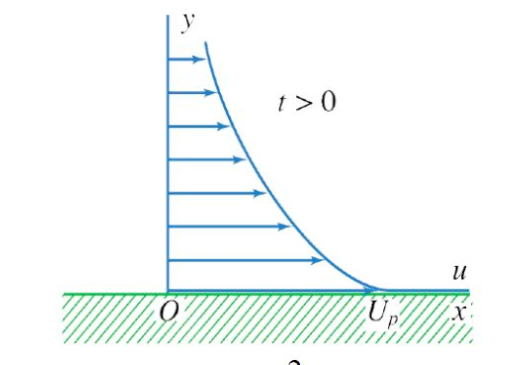
\includegraphics[width = 0.4\textwidth]{img/StokesProb1.png}
\caption{Diagram of the first Stokes problem.}
\label{fig:StokesProb1}
\end{figure}

In this case, we consider a plate moving horizontally with velocity $U_p$ as in \fref{fig:StokesProb1} with the diffusion equation  \[ \dpd{u}{t} = ν \dpd[2]{u}{y} \] and with boundary conditions $u(0,t) = U_p$ for $t > 0$ and $u(∞, t) = 0$.

If we put a scale $y = δ \tilde{y}$ with δ the thickness of the boundary layer, $u = U_p \tilde{u}$ and replacing $t = \sfrac{x}{U_p} \tilde{t}$ we can see that
\[
\frac{U_p^2}{x} \dpd{\tilde{u}}{t} = ν \frac{U_p}{δ^2} \dpd[2]{\tilde{u}}{\tilde{y}} \implies
δ \sim \sqrt{\frac{νx}{U_p}} = x \sqrt{\frac{1}{\rey_x}}
\] with $\rey_x = \sfrac{Ux}{ν}$.

This indicates that the height at which the movement has propagated upwards approximately scales like $\sqrt{\sfrac{νx}{U_p}}$, which is interesting as it gives us a variable thickness for the boundary layer. However, how does the flow look like there? To answer that we will go to the Stokes second problem.

\subsection{Stokes second problem}

We will consider a semi-infinite plane of fluid, with the bottom plate oscillating with velocity $u_p \cos ωt$. We have unidirectional so $v = 0$ (no vertical motion) and then we have the diffusion equation \[ \dpd{u}{t} = ν \dpd[2]{u}{y} \] with some bizarre boundary conditions, $u(0,t) = u_p \cos ωt$ and $u(∞,t) \to 0$.

This is a kind of a harmonically forced problems, which in our case means that the functions are sinusoid oscillations.

We can solve this problem by the ansatz $u = \hat{u}(y) \cos (ωt + φ) = \hat{u}(y) e^{\imath ω t} + c.c.$ (complex conjugate) which is a way of taking into account the phase with $\hat{u}(y)$ being a complex function. Now the equation becomes \begin{align*}
\imath ω \hat{u} e^{iωt} &= ν \dod[2]{\hat{u}}{y} e^{\imath ω t} \\
\frac{\imath ω}{ν} \hat{u} &= \dod[2]{\hat{u}}{y}
\end{align*} so that the solution is \[ \hat{u}(y) = A e^{\sqrt{\frac{\imath ω}{ν}} y} + B e^{-\sqrt{\frac{\imath ω}{ν}} y} = B e^{\frac{1}{2}\sqrt{\frac{2ω}{ν}} y} e^{\frac{\imath}{2}\sqrt{\frac{2ω}{ν}} y} + A e^{- \frac{1}{2}\sqrt{\frac{2ω}{ν}} y} e^{- \frac{\imath}{2}\sqrt{\frac{2ω}{ν}} y} \]

To have $\hat{u}(∞) = 0$ we need $B = 0$, and to have $u(0) = U_p$ we need $A = U_p$. Therefore, the final solution will be \[ u(y,t) = U_p e^{-\sqrt{\frac{ω}{2ν}} y} \cos \left(ωt - \sqrt{\frac{ω}{2ν}} y\right)\]

So we find that we have oscillations with exponentially decaying amplitude and height-dependent phase. For fluid mechanics, the penetration length $δ$ scales like $\sqrt{\frac{ν}{ω}}$. This makes sense as it is simlar to what we had with the Stokes first problem.

% Draw the cone thing.

So, in general, diffusion layers stay very small when $ν$ is small. So, for high Reynolds numbers the moment does not have time to diffuse into the flow. Therefore, we will be able to consider any flow at high Reynolds numbers as flows with vorticity concentrated on special points (vortices), filaments and close to the boundary. Therefore, we will solve for potential flow everywhere except in those special parts.

In this layer, the streamwise velocity is much larger than the normal velocities, and also the gradient of the streamwise velocity in the normal direction is going to be really high.

First question is thickness of the boundary layer. Based on the other problems (1st stokes problem) we know that the diffusion goes like $δ \sim \sqrt{νt}$. How does that diffuse in space? We can do dimensional analysis (slides) and then $δ(x) \sim \sqrt{\frac{νx}{U}}$. In the slides $\rey_x = \frac{Ux}{ν}$.

\subsection{Matched asymptotic expansion}

\begin{figure}[hbtp]
\centering
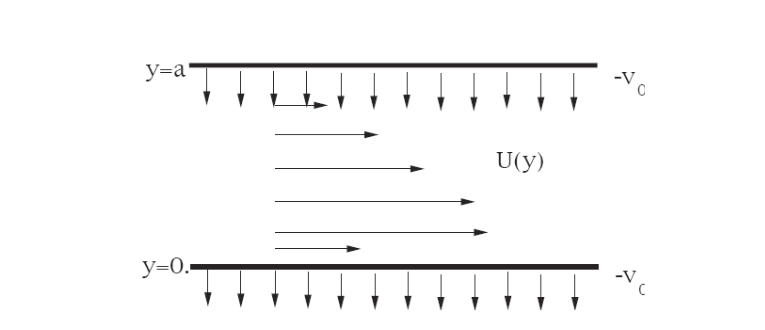
\includegraphics[width = 0.8\textwidth]{img/PouseilleFlowVerticalFlux.png}
\caption{A 2D channel flow from left to right due to an imposed pressure gradient with suction at the lower wall and blowing at the upper.}
\label{fig:PouseilleChannel}
\end{figure}

How does the flow look in that boundary layer? For that we need the method of matched asymptotic expansion.

An example problem is Pouseille flow in a channel with a uniform flux through the channel walls. Looking for a streamwise indepedent solution $\vu(x,y,z) = U(y) \ve_x + V(y) \ve_y$. With continuity we have $\pd{v}{y} = 0$ so $V(y) = V_0$.

We have the $y$ momentum equaiton which simplifies to $0 = \pd{p}{y}$ an therefore $p(x) = -k x + P_0$. In the $x$ momentum we find \[ -v_0 \dpd{U}{y} = \frac{k}{ρ} + ν \dpd[2]{U}{y} \] and with the boundary conditions we have that \[ U(y) = \frac{ka}{ρv_0} \left( - \frac{y}{a} + \frac{1 - e^{-\frac{v_0y}{ν}}}{1 - e^{-\frac{v_0a}{ν}}} \right) \]

If we nondimensionalize the equation with light blowing/suction ($\rey \ll 1$) we would still get something similar, with the first term of the asymptotic expansion of the exact solution.

However, in the case with $\rey \gg 1$ things change a little bit. From non-dimensionalization we get \[ ε u'' + u' + 1 = 0 \] with $ε = \sfrac{1}{\rey} \ll 1$. There is an issue: the term $εu''$ is negligible and solving with $u(0) = u(1) = 0$ we get a solution $u(y) = 1 - y$, which is not compatible with those conditions. However, $1 - y$ almost the exact solution except for the region near to the lower wall.

We can rescale close to $y = 0$ with $y = δ\tilde{y}$. Therefore, we can change dimensions again in the non-dimensionalized equations so that \[ε \frac{1}{δ^2} \dod[2]{\tilde{U}}{\tilde{y}} + \frac{1}{δ} \dod{\tilde{U}}{\tilde{y}} + 1 = 0 \]

Applying dominant balance we need $δ = ε$ and the equation becomes \[ \od[2]{\tilde{U}}{\tilde{y}} + \od{\tilde{U}}{\tilde{y}} = 0 \implies \tilde{U}(y) = A(1- e^{-\tilde{y}}) \] imposing the boundary condition $\tilde{U}(0) = 0$. Now we only need to match that to the previous solution we got $U =1 - y$: \[ \lim_{y \to 0} U(y) = \lim_{\tilde{y} \to ∞} \tilde{U}(\tilde{y}) \] and therefore we get $A = 1$.

That gives us a solution $\tilde{U}$. When $\tilde{y}$ goes too high, we are almost out of the boundary layer, so we match there the solutions. There's a typo and $\tilde{U} = A(1 - e^{-\tilde{y}})$ and a composite solution \[ U_\text{composite} = U(y) + \tilde{U}(\sfrac{y}{ε}) - U(0) \]

\section{General 2D flow with boundary layers}

We will apply this method to 2D flow:
\begin{align*}
∂_x u + ∂_y v &= 0 \\
(u∂_x + v ∂_y)u &= - \frac{1}{ρ} ∂_x p + ν Δu \\
(u∂_x + v ∂_y)v &= - \frac{1}{ρ} ∂_y p + ν Δv
\end{align*}

Now we make that non-dimensional. We say that $u = U_∞ \tilde{u}$, $u$ goes at the velocity of the free steam. If the boundary layer is small, there's a lubrication assumption so we set an unknown gauge $v = V \tilde{v}$.  Similary, $x = L \tilde{x}$, $y = δ \tilde{y}$ and $p = p_0 + P \tilde{p}$. The equations then are transformed. For the first, we have
\[ \frac{U}{L} ∂_{\tilde{x}} \tilde{u} + \frac{V}{δ} ∂_{\tilde{y}} \tilde{v} = 0 \] and applying dominant balance we set both terms to be of the same order, so the gauge $V$ is defined as $V = \frac{Uδ}{L}$.

For the momentum equations, we will have
\[ \frac{U^2}{L}\left( \tilde{u}∂_{\tilde{x}} \tilde{u} + \tilde{v} ∂_{\tilde{y}}\tilde{u} \right)= - \frac{P}{ρL} ∂_{\tilde{x}} \tilde{p} + ν\left( \frac{U}{L^2} ∂_{\tilde{x}}^2 \tilde{u} + \frac{U}{δ^2} ∂_{\tilde{y}}^2 \tilde{u} \right) \]

In the second derivatives, the $∂_x^2$ term is not going to be significant compared to the other one with $\frac{U}{δ^2}$, so that we find that \[ \frac{δ}{L} \sim \sqrt{\frac{ν}{UL}} = \sqrt{\rey} \] so that the boundary layer will be considerably thin. This is considerably bad for computational methods, as the mesh needs to account for a large $x$ scale but also modeling the behavior on the boundary layer of very small size in the perpendicular direction.

In the meantime, we got the pressure gauge as $P = ρU^2$. For the second momentum equation, we have
\[\frac{UV}{L}\left(\tilde{u}∂_{\tilde{x}} \tilde{v} + \tilde{v} ∂_{\tilde{y}} \tilde{v} \right) = - \frac{P}{ρδ} ∂_{\tilde{y}} \tilde{p} + ν \left( \frac{V}{L^2} ∂_{\tilde{x}}^2 \tilde{v} + \frac{V}{δ^2} ∂_{\tilde{y}}^2 \tilde{v}  \right)\]

In this case, we cet that the pressure gradient is dominant in the $y$ direction. The final equation system is
\begin{align*}
∂_{\tilde{x}} \tilde{u} + ∂_{\tilde{y}} \tilde{v} &= 0 \\
\tilde{u} ∂_{\tilde{x}} \tilde{u} + \tilde{v} ∂_{\tilde{y}} \tilde{u} &= - ∂_{\tilde{x}} \tilde{p} + ∂^2_{\tilde{y}} \tilde{u} \\
∂_{\tilde{y}} \tilde{p} &= 0
\end{align*}

So what we have is almost lubrication, but we also have advection. The important issue is the fact that the pressure does not vary in the boundary layer. For example, in aerodynamics, it allows to compute lift (which depends on pressure) just by using Euler equations: despite the fact that those not work in the boundary layer, the solution for the pressure they give is valid as it does not change along the boundary layer.

We need to impose boundary conditions now. We will focus on boundary layer in a flat plate. The Euler solution is $\vU = U_∞ \ve_x$, with a constant pressure. That kills the pressure gradient in the equation (asymptotic matching: $\tilde{p}(\tilde{y} \to ∞) = \bar{p}(\bar{y} \to 0) = p_\text{atm}$ where $\bar{p}$ is the pressure from the Euler equation).

We also have no-slip and no penetration conditions, so $\tilde{u} = \tilde{v} = 0$ on $\tilde{y} = 0$, and finally the asymptotic matching condition $\tilde{u}(\tilde{y} \to ∞) = \bar{u}(\bar{y} \to 0) = 1$ (we are using the appropriate gauge).

Now we use the self-similar approach to solve the equation. But before that we are going to use a trick for 2D, which is using a streamfunction: there exists a function $ψ$ such that $u = ∂_y ψ$ and $v = - ∂_xψ$. The continuity equation is therefore automatically satisfied and the momentum equation becomes (dropping tildes) \[ \dpd{ψ}{y} \frac{∂^2ψ}{∂x∂y} - \dpd{ψ}{x} \dpd[2]{ψ}{y} = \dpd[3]{ψ}{y} \] with boundary conditions \begin{align*}
∂_x ψ (y = 0) &= 0 &∀x \\
∂_y ψ (y = 0) &= 0 \\
∂_y ψ (y \to ∞) &= 1
\end{align*}

Integrating the first one, we have $ψ(y = 0) = 0$. With the third one, $ψ(y \to ∞) = y$ forgetting about that thing of having care when integrating limits.

For the self-similar solution, we search for a function $F(ψ,x,y)$. We define $ψ = ψ_* \hat{ψ}$ with $ψ_*$ a dilation coefficient. Similarly, we define $x = x_* \hat{x}$ and $y = y_* y$. Injecting this in the equations we have
\[ \frac{ψ_*^2}{x_* y_*^2} \dpd{\hat{ψ}}{\hat{y}} \frac{∂^2\hat{ψ}}{∂\hat{x} ∂\hat{y}} - \frac{ψ_*^2}{x_* y_*^2}\dpd{\hat{ψ}}{\hat{x}} \dpd[2]{\hat{ψ}}{\hat{y}} = \frac{ψ_*}{y_*^3} \dpd[3]{\hat{ψ}}{\hat{y}} \] and in the boundary conditions
\begin{align*}
ψ_* \hat{ψ} (y_* \hat{y} = 0) &= 0 \\
\frac{ψ_*}{y_*} \dpd{\hat{ψ}}{\hat{y}} (y_* \hat{y} = 0) &= 0 \\
ψ_* \hat{ψ}(y_* \hat{y} \to ∞) &= y_* \hat{y}
\end{align*}

For the hat problem to be the same as the original problem, we needto have $ψ_* = y_*$ and $\frac{ψ_*^2}{x_*y_*^2} = \frac{ψ_*}{y_*^3}$ so that $x_* = y_*^2$. So we will consider the equation $G(\sfrac{ψ}{\sqrt{x}}, x, \sfrac{y}{\sqrt{x}}) = 0$. I am hungry. Changing that we have that $G(\sfrac{\hat{ψ}}{\sqrt{\hat{x}}},x_* \hat{x}, \sfrac{\hat{y}}{\sqrt{\hat{x}}})$ and therefore $ψ = \sqrt{x} f(\sfrac{y}{\sqrt{x}})$. We will call $η ≝ \sfrac{y}{\sqrt{x}}$. This is more or less like a separation of variables but more general.

Now we need to rephrase that equation with our new set of variables. Please god no. All the coefficients disappear and we will drop the hats. First we solve the derivatives separately:
\begin{align*}
\dpd{η}{y} &= \frac{1}{\sqrt{x}} \\
\dpd{η}{x} &= - \frac{1}{2} \frac{y}{x \sqrt{x}} = - \frac{η}{2x} \\
\dpd{ψ}{y} &= \sqrt{x} f'(η) \dpd{η}{y} = f' \\
\frac{∂^2ψ}{∂x∂y} &= f''(η) \dpd{η}{x} = - \frac{ηf''}{2x} \\
\dpd{ψ}{x} &= \frac{1}{2\sqrt{x}} f + f'(η) \dpd{η}{x} = \frac{1}{2\sqrt{x}}( f -ηf') \\
\dpd[2]{ψ}{y} &= \frac{f''(η) }{\sqrt{x}} \\
\dpd[3]{ψ}{y} &= \frac{f'''(η)}{x}
\end{align*} and then the equation becomes
\begin{align*}
 - \frac{f'ηf''}{2x} - \frac{1}{2 x} (f - η f')f'' &= \frac{f'''}{x} \\
 -ff'' &= 2f'''
 \end{align*}

This is called the Blasius equation. We need boundary conditions, and when $y = 0$ $η = 0$, and same with $y = ∞ \implies η = ∞$, so that $f(0) = 0$, $f'(0) = 0$ and $f \to η$ when $y \to ∞$.

The solution is an exponential relaxation on $u = f'$.

On the practical level, we have to define the layer thickness. There's no unique definition.  Slides. Displacement thickness making the flux equal in both displaced and flat probdiles. Last one is momentum, but isntead of conserving mass flux you consider momentum flux.

\chapter{Vorticity: Inviscid and potential flow}

This chapter will be dedicated to the study of tools for understanding vorticity. On a plane, the vorticity equation of ω  is given by \[ \dpd{ω}{t} + u \dpd{ω}{x} + ν \dpd{ω}{y} = ν \left(\dpd[2]{ω}{x} + \dpd[2]{ω}{y}\right) \] and in the axisimmetric case we have \[
\dpd{ω}{t} + u \dpd{ω}{z} + ν \dpd{ω}{r} = ν \left(\dpd[2]{ω}{z} + \dpd[2]{ω}{r} + \frac{1}{r} \dpd{ω}{r} - \frac{ω}{r^2} \right) \]

Given a vorticity field $ω(x,y)$ one can use Biot-Savart induction and the streamfunction to obtain\footnote{Let's not ask about convergence issues...}
\begin{align*}
Ψ(x,y) &= - \frac{1}{4π} \iint_D ω(x', y') \log \left((x' - x)^2 + (y' -y)^2 \right) \dif x' \dif y' \\
u(x,y) &= ∂_y ψ = \frac{1}{2π} \iint_D\frac{(y'-y) ω(x',y')}{(x' - x)^2 + (y' - y)^2} \dif x' \dif y' \\
v(x,y) &= -∂_x ψ = \frac{1}{2π} \iint_D\frac{(x'-x) ω(x',y')}{(x' - x)^2 + (y' - y)^2} \dif x' \dif y'
\end{align*}

We can have different types of vortices, such as a point vortex \[ ω(x,y) = k δ(x -x_1)δ(y - y_1)\] or a vortex ring \[ ω_φ(x, r) = γδ(x) δ(r - R)\]

Some interesting properties for vortices: two vortices with different sign travel with the same velocity, depending on their separation (closer imply faster). Two vortexes of same sign will rotate around the center and merge eventually.

When there's shear and vorticity, the vorticity is tilted towards the direction of the shear.Also, if there is convergence in a plane of flows, it goes upwards (stretching). There is also a term $\frac{1}{ρ} \od{ρ}{t}$ which is barocycaslkdas dependence and very important in metereology but not so much for us.

In vorticity fields we have $\dv \vec{ω} = 0$, so  vortex lines need to be either closed, infinite or touch the boundaries. In circulation, we integrate tarngential velocity along the contour, and that's equal to the flux of vorticity. But very difficult to use this.

\section{Inviscid fluid}

Inviscid flow is governed by the Euler equations which we recall here as \begin{align*}
\dod{ρ}{t} + ρ \dv \vU &= 0 \\
ρ \frac{\Dif\vU}{t} &= ρ \vF - ∇p
  \end{align*}

\section{Potential flow}

Potential flow is approximated with vorticity zero. In general, inviscid regions are irrotational but there are situations where they can be rotational (e.g., solid body rotation). This flow is governed by the potential $\appl{φ}{ℝ^3}{ℝ}$ and the equations
\begin{align*}
Δφ &= 0 \\
\vU &= ∇φ \\
\dpd{φ}{t} + \frac{p}{ρ} + \frac{U^2}{2} + φ &= C(t)
\end{align*}

\begin{table}[hbtp]
\centering
\begin{tabular}{p{6cm}cc}
\toprule
\textbf{Type} & \textbf{Potential} φ & \textbf{Streamfunction} ψ  \\ \toprule
Planar & $Vr \cos θ $ &$Vr \sin θ$ \\
Source/sink at origin w/ volume flow rate $\frac{V}{L}$ &  $\frac{V}{L2π} \ln r$ & $\frac{V}{L2π}θ $ \\
Line vortex & $\frac{Γ}{2π}θ$ & $- \frac{Γ}{2π} \ln r$ \\
Doublet (source and sink) strength $K$ & $-K\frac{\sin θ}{r}$ & $K \frac{\cos θ}{r}$ \\ \bottomrule
\end{tabular}
\caption{Some examples of potential and streamfunctions for flows. Note that the cartesian functions (around the origin $(x_0, y_0)$) can be obtained by replacing, as usual, $r = \sqrt{(x - x_0)^2 + (y - y_0^2)}$ and $θ = \arctan \frac{y - y_0}{x -x_0}$.}
\label{tab:FlowExamples}
\end{table}

Several examples of streamfunction and potential combinations are shown in \fref{tab:FlowExamples}. These can be combined by simply summing them. E.g., a bathtub vortex is a line vortex and a sink, so we have just to add both.

Another interesting example is that one can obtain the flow along a sphere of radius $a$ by combining a doublet and a planar stream, so that \begin{align*}
φ &= U_∞r \cos θ + K \frac{\cos θ}{r} \\
ψ &= U_∞r \sin θ - K \frac{\sin θ}{r}
\end{align*}

If we assume that around the body border we have $ψ = 0$ (that is, when $r = a$) so we set $K = U_∞a^2$. Replacing and diffferentiating the streamfunction we get the velocity \begin{align*}
U_r &= \frac{1}{r} \dpd{ψ}{θ} = U_∞ \cos θ \left(1 - \frac{a^2}{r^2}\right) \\
U_θ &= - \dpd{ψ}{r} = - U_∞ \sin θ \left(1 + \frac{a^2}{r^2}\right)
\end{align*} which funnily enough gives no penetration in the boundary $r =a$ but gives slip condition as $U_θ(r = a) ≠ 0$.

The presure profile is obtained by applying the Bernoulli equation, comparing the pressure far away downstream and in the surface of the sphere (angle θ) so that
\[ p_∞ + \frac{1}{2} ρU_∞^2 = p(a, θ) + \frac{1}{2} ρ U_θ^2 \implies p(a,θ) = p_∞ + \frac{ρU_∞^2}{2} (1 - 4 sin^2 θ) \]

\section{Complex analysis of flows}

Now we enter into the part where mathematics are useful. Given the definitions of potential flow and streamfunction, we had that \begin{align*}
U_x &= \dpd{φ}{x} = \dpd{ψ}{y} \\
U_y &= \dpd{φ}{y} = - \dpd{ψ}{x}
\end{align*}

This means that, if we consider the complex function \[ f(x + \imath y) = φ(x,y) + \imath ψ(x,y) \] it is a holomorphic function as it satisfies Cauchy-Riemman equations! Furthermore, if we derive (in the complex sense) $f$ we get the velocity field: \[ f'(z) = \frac{1}{2} \left( \dpd{f}{x} - \imath \dpd{f}{y} \right) = \frac{1}{2} \left(U_x - \imath U_y - \imath \left( U_y  + \imath U_x\right) \right ) = U_x - \imath U_y \]

\begin{table}[hbtp]
\centering
\begin{tabular}{p{5cm}ccc}
\toprule
\textbf{Type} & \textbf{Potential} φ & \textbf{Streamfunction} ψ & \textbf{Complex form}  \\ \toprule
Planar (angled α) & $Vr \cos (θ - α) $ &$Vr \sin (θ - α)$ & $Ue^{-\imath α} z$  \\
Source/sink at $z_0$ w/ volume flow rate $\frac{V}{L}$ &  $\frac{V}{L2π} \ln r$ & $\frac{V}{L2π}θ $  & $\frac{V}{Lwπ}\log (z - z_0)$ \\
Line vortex & $\frac{Γ}{2π}θ$ & $- \frac{Γ}{2π} \ln r$ & $- \frac{\imath Γ}{2π} \log (z - z_0)$ \\
Doublet (source and sink) strength $K$ & $-K\frac{\sin θ}{r}$ & $K \frac{\cos θ}{r}$ & $- \frac{K}{z - z_0}$ \\ \bottomrule
\end{tabular}
\caption{Some examples of potential and streamfunctions for flows with the corresponding complex functions associated. Note that we can always rotate the flow multiplying by $e^{-\imath α}$}
\label{tab:FlowExamples}
\end{table}

With this we can come back to the example of the flow around a circular body. But take into account that we can also add a line vortex, which is harmonic on $ℝ^2 \minuszero$ (funny things that happens in non-simply connected domains) and therefore our general solution is \[ f(z) = U_∞ \left(z + \frac{a^2}{z} \right) - \frac{\imathΓ}{2π} \log \frac{z}{a} \]

With $-1 < \frac{Γ}{4πU_∞ a} < 0$ we have the pressure profile \[ p(a, θ) = \frac{1}{2}ρU_∞^2 \left(1 - 4 \left(\sin θ - \frac{Γ}{4πU_∞a}\right)^2 \right)\] which gives a lift force! This is the Magnus effect that can be seen in football.

\subsection{Conformal maps}

Conformal maps are transformations of the complex plane that preserve local angles. Mathematically, a map $\appl{h}{U ⊆ ℂ}{ℂ}$ is conformal if and only if it is holomorphic and its derivative is everywhere non-zero on $U$.

These maps allow the transformation of the domain and might serve to simplify the study of potentials: if we have a potential $f(z)$ that is difficult, we can try to find a conformal map $Z = h(z)$ and study the simplified potential $F(h(z))$.

\begin{figure}[hbtp]
\centering
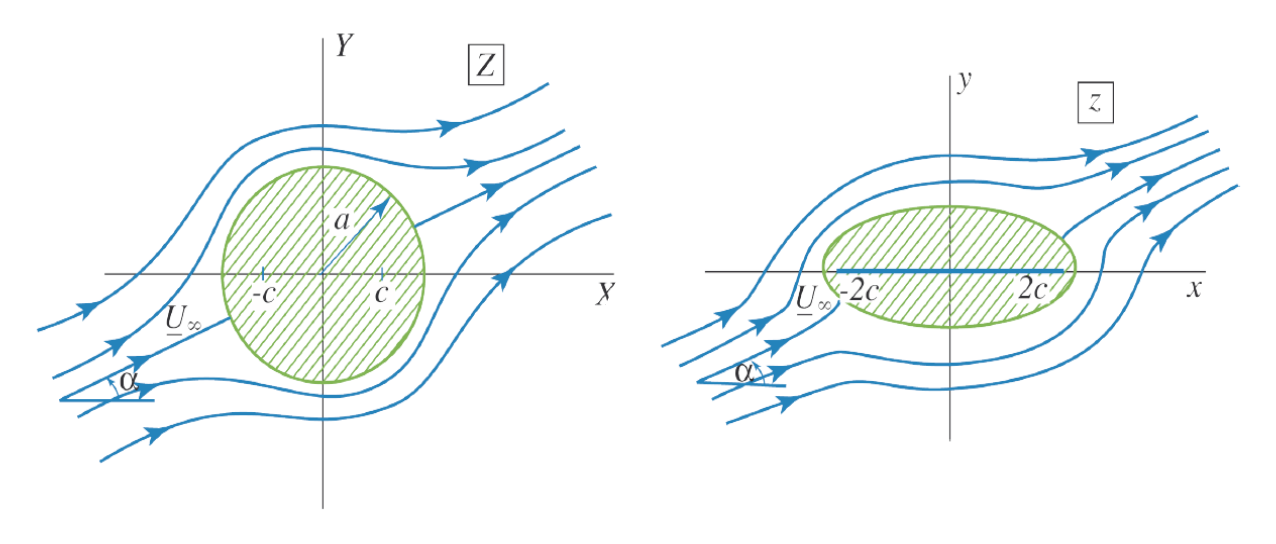
\includegraphics[width=0.8\textwidth]{img/Joukowski.png}
\caption{Joukowski transform.}
\label{fig:Joukowski}
\end{figure}

One of these useful maps is the Joukowski transform, defined as \[ z = Z + \frac{c^2}{Z} \] which maps a circle of radius $c$ to a plane of length $4c$, and circles of radius $a > c$ to ellipses of major axis $2c$ (\fref{fig:Joukowski}). The inverse transform is not unique, but we choose the positive branch to conserve the physics:
\[ Z = \frac{z + \sqrt{z^2 - 4c^2}}{2} \]

With this, we can study the flow around a plate of length $4c$, with the fluid coming at an angle $α$ with velocity $U_∞$. The potential will be defined as $f(z) = U_∞ e^{-\imath α} z$, which on the transformed $Z$ plane will become
\[ F(Z) = U_∞ \left(Z e^{-\imath α} + \frac{c^2}{Z} e^{\imath α}\right) - \frac{\imath Γ}{2π} \log Z \] where the second term is the undetermined circulation around the plate (recall that the domain is not simply connected and we have multiple possible solutions).

There we could identify the points with velocity $0$ as those where $F'(Z) = 0$ and where $Z = a e^{\imath θ}$ (that is, those on the circle). It seems that can be done by replacing directly $Z = ae^{\imath θ}$ and then deriving with respect to θ but I am not that convinced about it.

We could apply the Kutta principle, which says that a body with a sharp trailing edge which is moving through a fluid will create about itself a circulation of sufficient strength to hold the rear stagnation point at the trailing edge. We can solve for circulation then assuming that the stagnation point is at $θ = 0$. This allows to get the lift force by $F_l = - ρ U_∞ Γ$ with ρ the density of the fluid.

\appendix


\chapter{Equations and other tools}

\section{Navier-Stokes}

Navier-Stokes equation model the flow velocity $\appl{u}{ℝ^3}{ℝ^3}$ of a fluid with density $ρ$ at pressure $p$ and viscosity $μ$, everything depending on time.

\(
\begin{aligned}
 x&:\ &\rho \left(\frac{\partial u_x}{\partial t} + u_x \frac{\partial u_x}{\partial x} + u_y \frac{\partial u_x}{\partial y} + u_z \frac{\partial u_x}{\partial z}\right) &= -\frac{\partial p}{\partial x} + \mu \left(\frac{\partial^2 u_x}{\partial x^2} + \frac{\partial^2 u_x}{\partial y^2} + \frac{\partial^2 u_x}{\partial z^2}\right) \\ & & &- \mu \frac{\partial}{\partial x} \left( \frac{\partial u_x}{\partial x} + \frac{\partial u_y}{\partial y} + \frac{\partial u_z}{\partial z} \right) + \rho g_x \\
 y&:\ &\rho \left(\frac{\partial u_y}{\partial t} + u_x \frac{\partial u_y}{\partial x} + u_y \frac{\partial u_y}{\partial y}+ u_z \frac{\partial u_y}{\partial z}\right) &= -\frac{\partial p}{\partial y} + \mu \left(\frac{\partial^2 u_y}{\partial x^2} + \frac{\partial^2 u_y}{\partial y^2} + \frac{\partial^2 u_y}{\partial z^2}\right) \\ & & &- \mu \frac{\partial}{\partial y} \left( \frac{\partial u_x}{\partial x} + \frac{\partial u_y}{\partial y} + \frac{\partial u_z}{\partial z} \right) + \rho g_y \\
 z&:\ &\rho \left(\frac{\partial u_z}{\partial t} + u_x \frac{\partial u_z}{\partial x} + u_y \frac{\partial u_z}{\partial y}+ u_z \frac{\partial u_z}{\partial z}\right) &= -\frac{\partial p}{\partial z} + \mu \left(\frac{\partial^2 u_z}{\partial x^2} + \frac{\partial^2 u_z}{\partial y^2} + \frac{\partial^2 u_z}{\partial z^2}\right) \\ & & &- \mu \frac{\partial}{\partial z} \left( \frac{\partial u_x}{\partial x} + \frac{\partial u_y}{\partial y} + \frac{\partial u_z}{\partial z} \right) + \rho g_z. \\
 Cont&:\ &  \frac{\partial \rho}{\partial t} + \frac{\partial \left(\rho u_x \right) }{ \partial x} + \frac{\partial \left(\rho u_y\right) }{ \partial y} + \frac{\partial \left(\rho u_z\right) }{ \partial z} &= 0
\end{aligned} \label{eq:NavierStokes:Cartesian} \)

Note that the third term of the left-hand sides is $\dv \vU$ which is zero on incompressible fluids.


Incompressible flow equations in cylindrical coordinates

\(
\begin{aligned}
 r&:\ & \rho \left(\frac{\partial u_r}{\partial t} + u_r \frac{\partial u_r}{\partial r} + \frac{u_{\phi}}{r} \frac{\partial u_r}{\partial \phi} + u_z \frac{\partial u_r}{\partial z} - \frac{u_{\phi}^2}{r}\right) &= -\frac{\partial p}{\partial r} + \mu \left(\frac{1}{r}\frac{\partial}{\partial r}\left(r \frac{\partial u_r}{\partial r}\right) +
 \frac{1}{r^2}\frac{\partial^2 u_r}{\partial \phi^2} + \right.\\ & & &\left. + \frac{\partial^2 u_r}{\partial z^2} - \frac{u_r}{r^2} -
 \frac{2}{r^2}\frac{\partial u_\phi}{\partial \phi} \right) + \rho g_r \\
 \phi&:\ & \rho \left(\frac{\partial u_{\phi}}{\partial t} + u_r \frac{\partial u_{\phi}}{\partial r} +
 \frac{u_{\phi}}{r} \frac{\partial u_{\phi}}{\partial \phi} + u_z \frac{\partial u_{\phi}}{\partial z} + \frac{u_r u_{\phi}}{r}\right) &= -\frac{1}{r}\frac{\partial p}{\partial \phi} + \mu \left(\frac{1}{r}\frac{\partial}{\partial r}\left(r \frac{\partial u_{\phi}}{\partial r}\right) +
 \frac{1}{r^2}\frac{\partial^2 u_{\phi}}{\partial \phi^2} + \right.\\ & & &\left. + \frac{\partial^2 u_{\phi}}{\partial z^2} + \frac{2}{r^2}\frac{\partial u_r}{\partial \phi}-\frac{u_{\phi}}{r^2}\right) + \rho g_{\phi} \\
 z&:\ & \rho \left(\frac{\partial u_z}{\partial t} + u_r \frac{\partial u_z}{\partial r} + \frac{u_{\phi}}{r} \frac{\partial u_z}{\partial \phi} +
 u_z \frac{\partial u_z}{\partial z}\right) &= -\frac{\partial p}{\partial z} + \mu \left(\frac{1}{r}\frac{\partial}{\partial r}\left(r \frac{\partial u_z}{\partial r}\right) +
 \frac{1}{r^2}\frac{\partial^2 u_z}{\partial \phi^2} + \right. \\ & & & \left.+ \frac{\partial^2 u_z}{\partial z^2}\right) + \rho g_z \\
 Cont&:\ & \frac{1}{r}\frac{\partial r u_r}{\partial r} + \frac{1}{r}\frac{\partial u_\phi}{\partial \phi} + \frac{\partial u_z}{\partial z} &= 0
\end{aligned} \label{eq:NavierStokes:Cylindrical}
\)

\section{Random physics facts}

At an interface with normal $\vn$ and curvature $\mathcal{C}$, two fluids will have an equilibrum of $σ_1 \vn - σ_2 \vn = γ\mathcal{C} \vn$, where $γ$ is the surface tension. More specifically, if the difference in pressure is $Δp$, the equation reads $Δp = - γ \left(\sfrac{1}{R_1} + \sfrac{1}{R_2}\right)$.

Ideal gas law: $PV = nRT$.

Reynolds number: $\mop{Re} = \frac{ρvL}{μ}$ with ρ density, $v$ speed, $L$ some kind of length, and $μ$ dynamic viscosity ($N·s/m^2$).

Rayleigh number controling buoyancy: $\mathrm{Ra} = \frac{α g ΔT x^3}{μ κ}$ with α thermal expansion coefficient, κ thermal diffusivity, $ΔT$ difference in temperature between the point and another place far from the surface of the object and $g$ is gravity.

The Froude number is defined as the ratio of flow intertia to external field so \[ \mop{Fr} = \frac{u_0}{\sqrt{g_0 l_0}}\] with $u_0$ characteristic flow velocity, $g_0$ characteristic external field (e.g., gravity) and $l$ a characteristic length.

Heat equation in cylindrical coordinates:
\begin{align*}
&ρc_p \left(\dpd{T}{t} + U \dpd{T}{r} + \frac{V}{r} \dpd{T}{θ} + W \dpd{T}{z} \right) = \\
&\qquad = μ \left[\left(\frac{1}{r} \dpd{W}{θ} + \dpd{V}{z}\right)^2 + \left(\dpd{W}{r} + \dpd{U}{z} \right)^2 + \left(r \dpd{}{r} \left(\frac{V}{r}\right) + \frac{1}{r} \dpd{U}{θ} \right)^2 \right] + \\
&\qquad κ
\left(\frac{1}{r} \dpd{}{r} \left(r \dpd{T}{r}\right) + \frac{1}{r^2} \dpd[2]{T}{θ} + \dpd[2]{T}{z} \right)
\end{align*} with $c_p$ the specific heat and κ the conductivity.

\section{Random math facts}

If $f'' = k^2 f$, then $f = c_1 e^{kx} + c_2 e^{-kx}$ with possibly $k ∈ ℂ$.

Divergence in cylindrical coordinates: \[ \dv (A_ρ, A_φ, A_z) = \frac{1}{ρ} ∂_ρ (ρA_ρ) + \frac{1}{ρ} ∂_φ A_φ + ∂_z A_x \]

For curl, $\curl (\curl \vv) = ∇ \dv \vv - Δ \vv$. Laplacian of a vector is the vector of the laplacian of every coordinate.

Also, $Δ^2 f = ∇^4 f= Δ(Δf) = \sum_i \sum_j \frac{∂^4f}{∂x_i^2 ∂x_j^2}$.

If $\vv = (v_1, \dotsc, v_n)$ is a vector field, then \begin{align*}
Δ\vv = ∇^2 \vv &= ∇\dv \vv - \curl(\curl \vv)\\
∇\vv &= (∇v_1, ∇v_2, \dotsc, ∇v_n) \text{  (Matrix)}
\end{align*}


Some rules:
\begin{align*}
                           \nabla (fg) &= f\nabla g + g\nabla f \\
           \nabla(\vec u \cdot \vec v) &= \vec u \times (\nabla \times \vec v) + \vec v \times (\nabla \times \vec u) + ( \vec u \cdot \nabla) \vec v + (\vec v \cdot \nabla )\vec u \\
               \nabla \cdot (f \vec v) &= f (\nabla \cdot \vec v) + \vec v \cdot (\nabla f) \\
   \nabla \cdot (\vec u \times \vec v) &= \vec v \cdot (\nabla \times \vec u) - \vec u \cdot (\nabla \times \vec v ) \\
              \nabla \times (f \vec v) &= (\nabla f) \times \vec v + f (\nabla \times \vec v) \\
  \nabla \times (\vec u \times \vec v) &= \vec u \, (\nabla \cdot \vec v) - \vec v \, (\nabla \cdot \vec u) + (\vec v \cdot \nabla) \, \vec u - (\vec u \cdot \nabla) \, \vec v
\end{align*}

Operators in cylindrical coordinates:
\begin{align*}
∇_cf &= \dpd{f}{r} \ve_r + \frac{1}{r} \dpd{f}{θ} \ve_θ + \dpd{f}{z} \ve_z \\
Δ_cf &= \frac{1}{r} \dpd{}{r} \left(r \dpd{f}{r} \right) + \frac{1}{r^2} \dpd[2]{f}{r} + \dpd[2]{f}{z} \\
\rot_c \vf &= \left(\frac{1}{r} \dpd{f_z}{θ} - \dpd{f_θ}{z}\right) \ve_r + \left(\dpd{f_r}{z} - \dpd{f_z}{r} \right) \ve_θ + \left(\frac{1}{r} \dpd{rf_θ}{r} - \frac{1}{r} \dpd{f_r}{θ} \right) \ve_z
\end{align*}

An integration trick $uu' = \frac{1}{2}(u^2)'$

Some integrals and derivatives
\begin{align*}
f(x) = a^x &\implies f'(x) = x' a^x \ln a \\
f'(x) = \frac{1}{x} & \implies f(x) = \ln \abs{x}
\end{align*}

Some trigonometric identities
\begin{align*}
\sin α \pm β &= \sin α \cos β \pm \cos α \sin β &
\cos α \pm β &= \cos α \cos β \mp \sin α \sin β \\
\tan α \pm β &= \frac{\tan α \pm \tan β}{1 \mp \tan α \tan β} \\
\sin^2 θ &= \frac{1 - \cos 2 θ}{2} &
\cos^2 θ &= \frac{1 + \cos 2θ}{2} \\
\sinh θ &= \frac{e^θ - e^{-θ}}{2} &
\cosh θ &= \frac{e^θ + e^{-θ}}{2}
\end{align*}

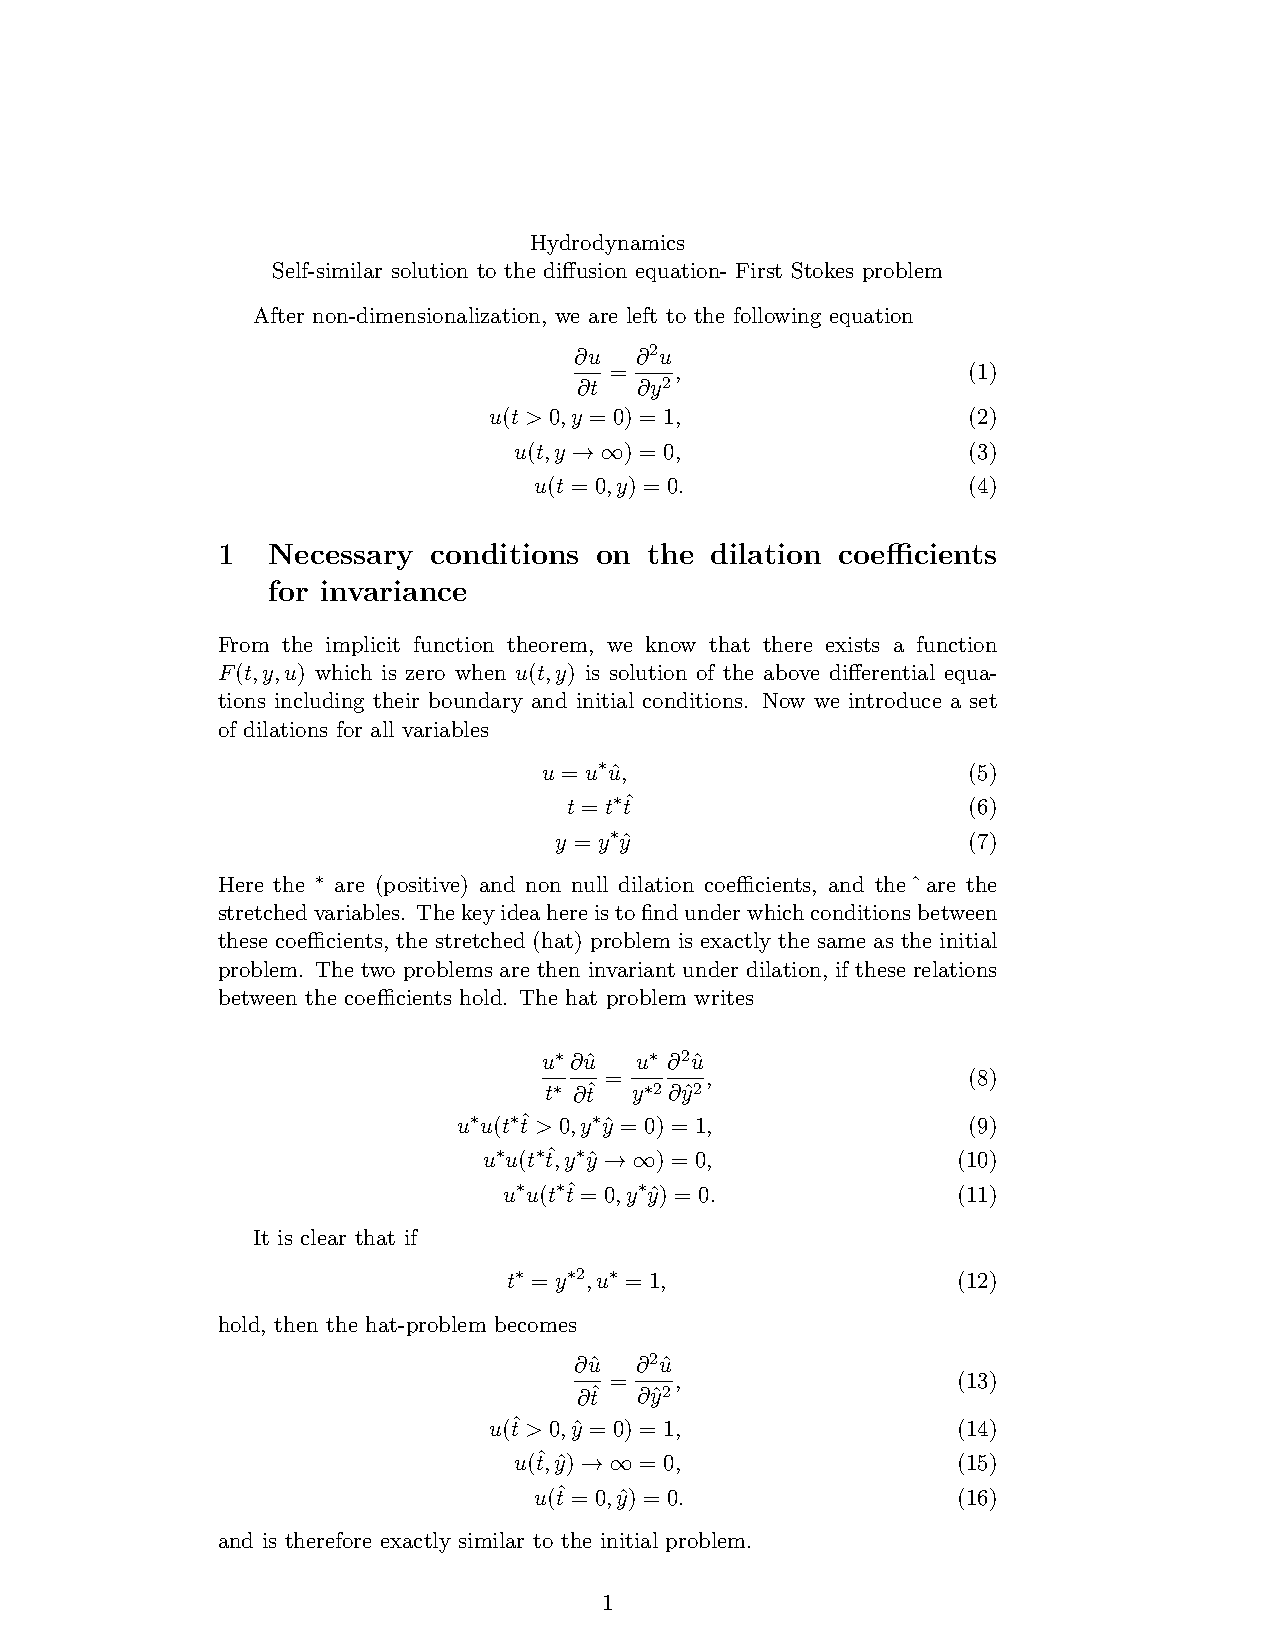
\includepdf[pages={1-},nup={2x2}]{pdf/_notediffusion.pdf}
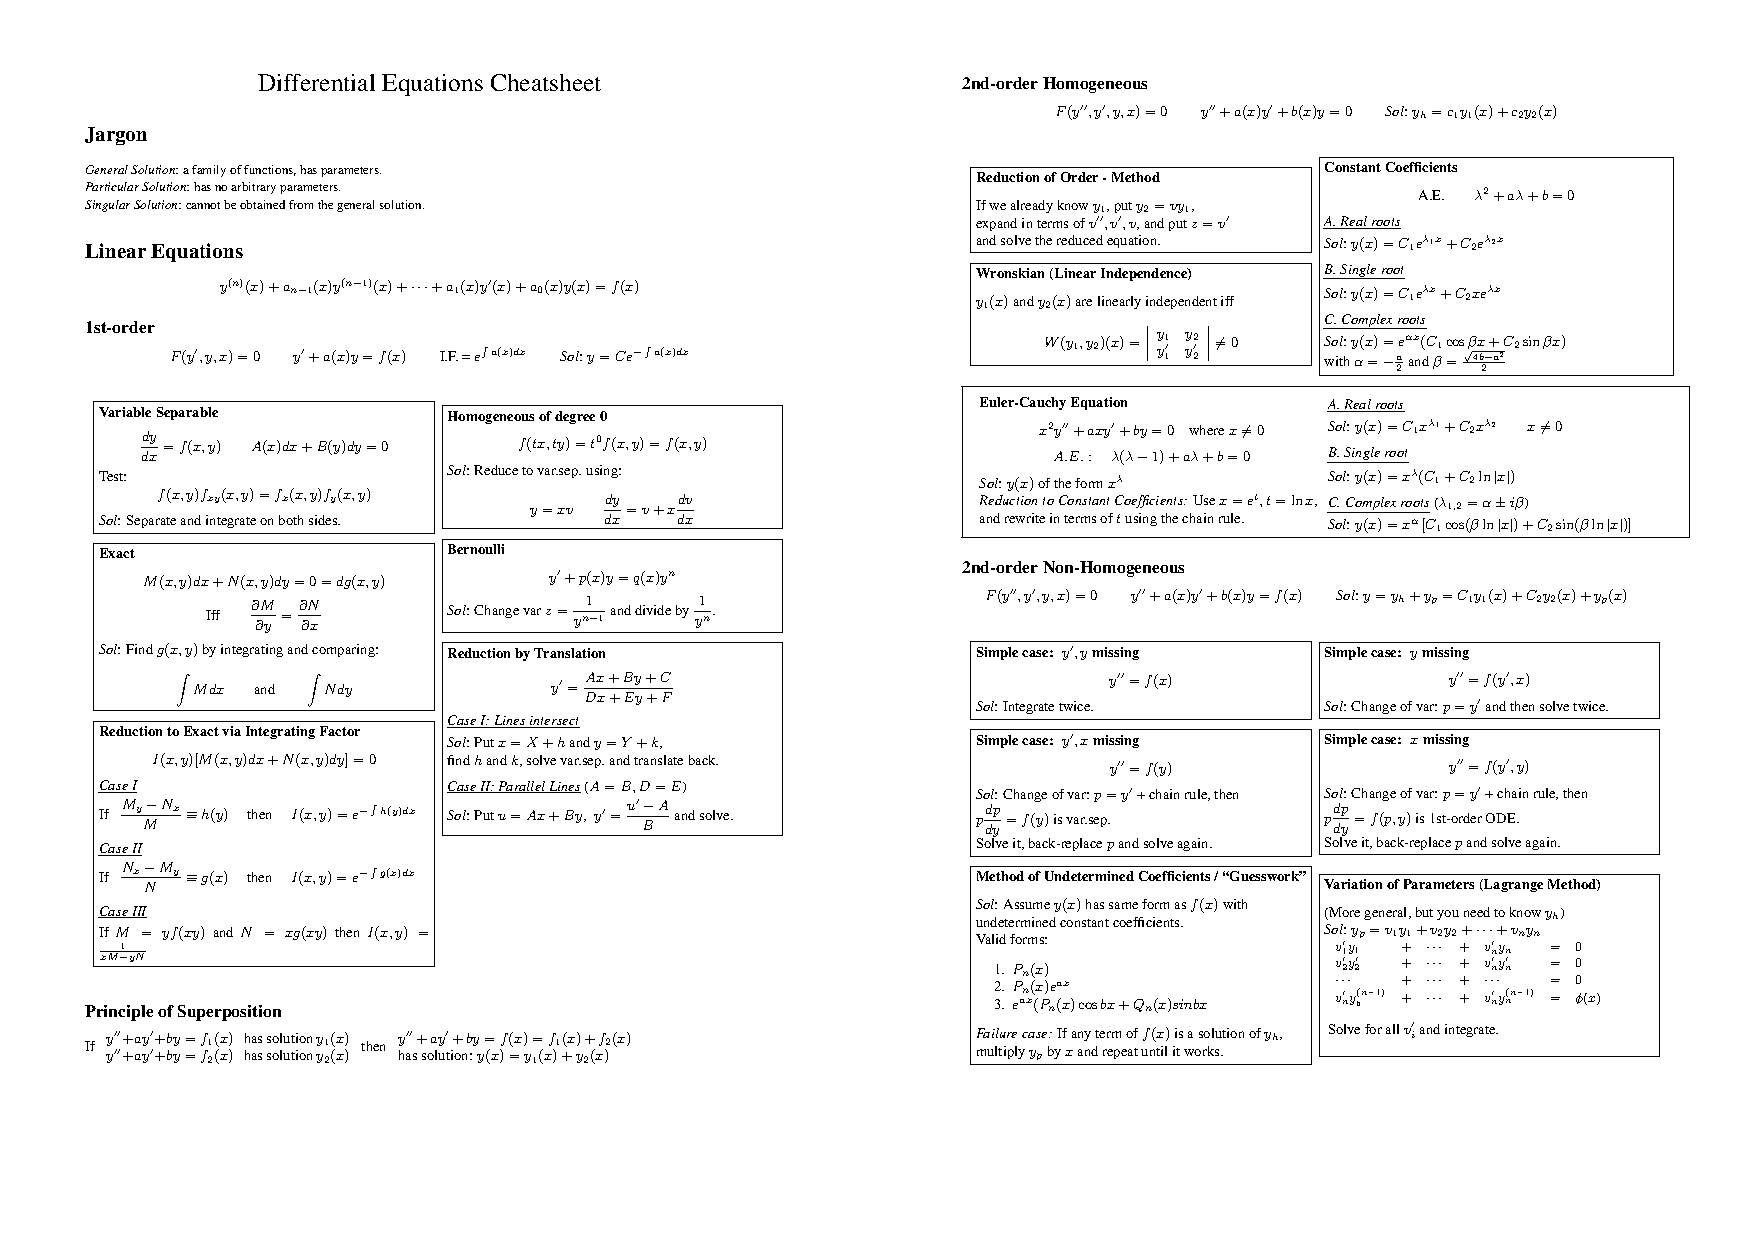
\includepdf[pages={1-},nup={1x2}]{pdf/_diffequs.pdf}
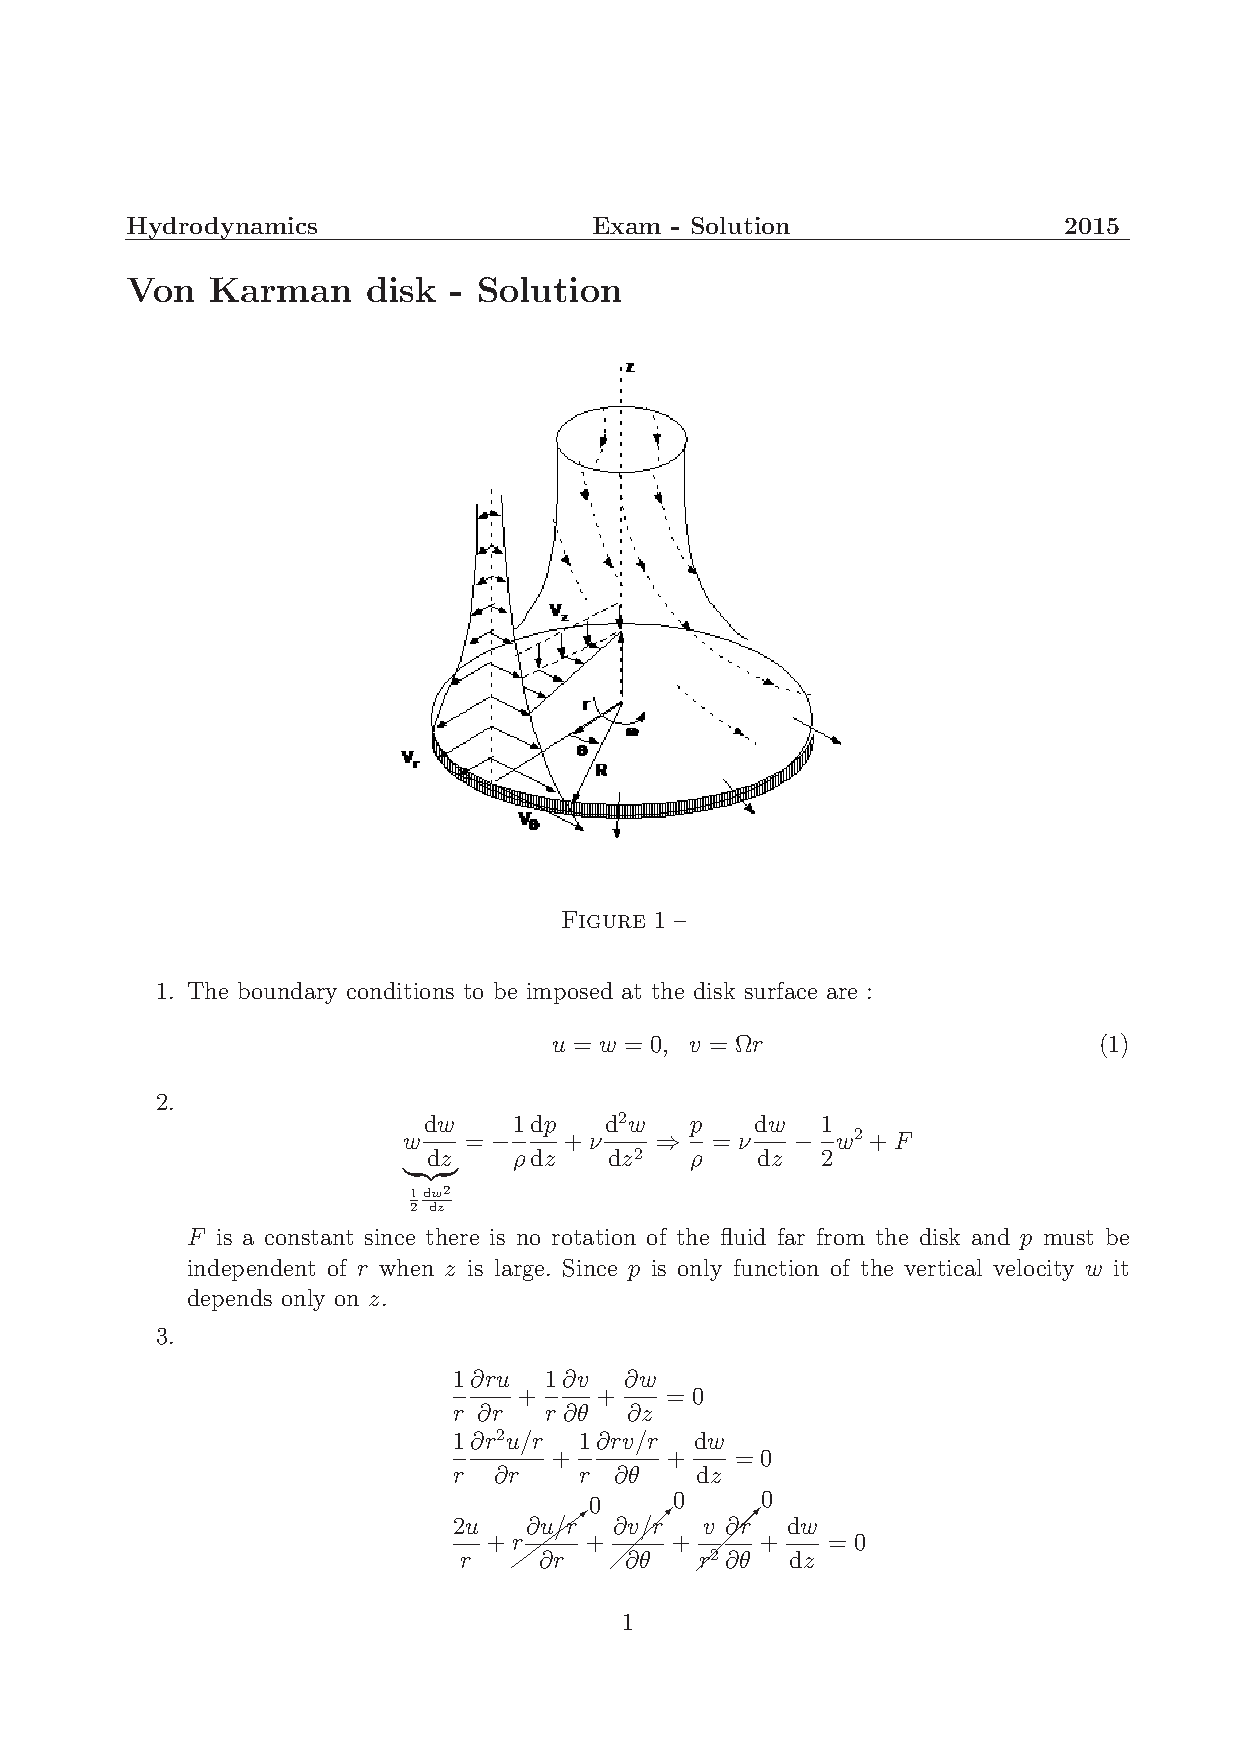
\includepdf[pages={1-},nup={2x2}]{pdf/_VKD2016Solution.pdf}
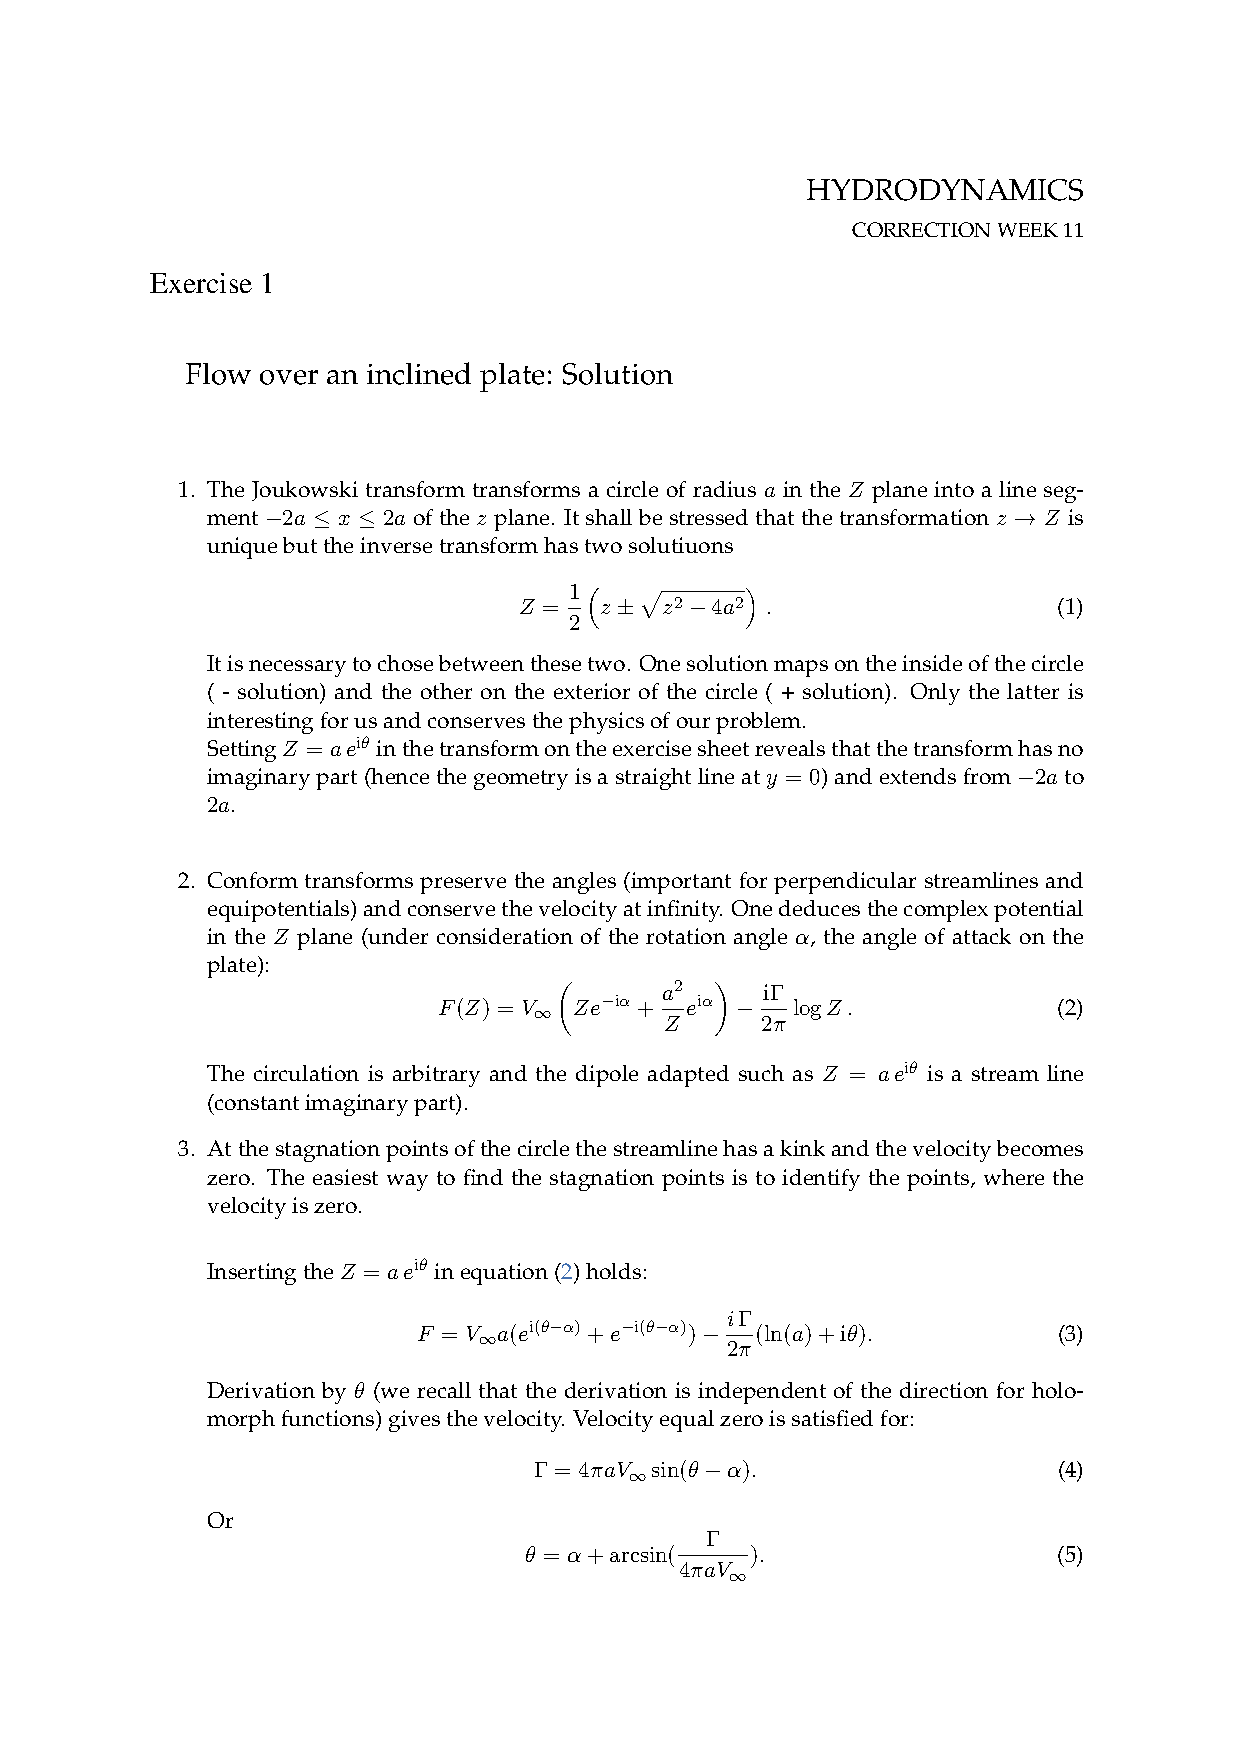
\includepdf[pages={1-},nup={2x2}]{pdf/_Transforms.pdf}
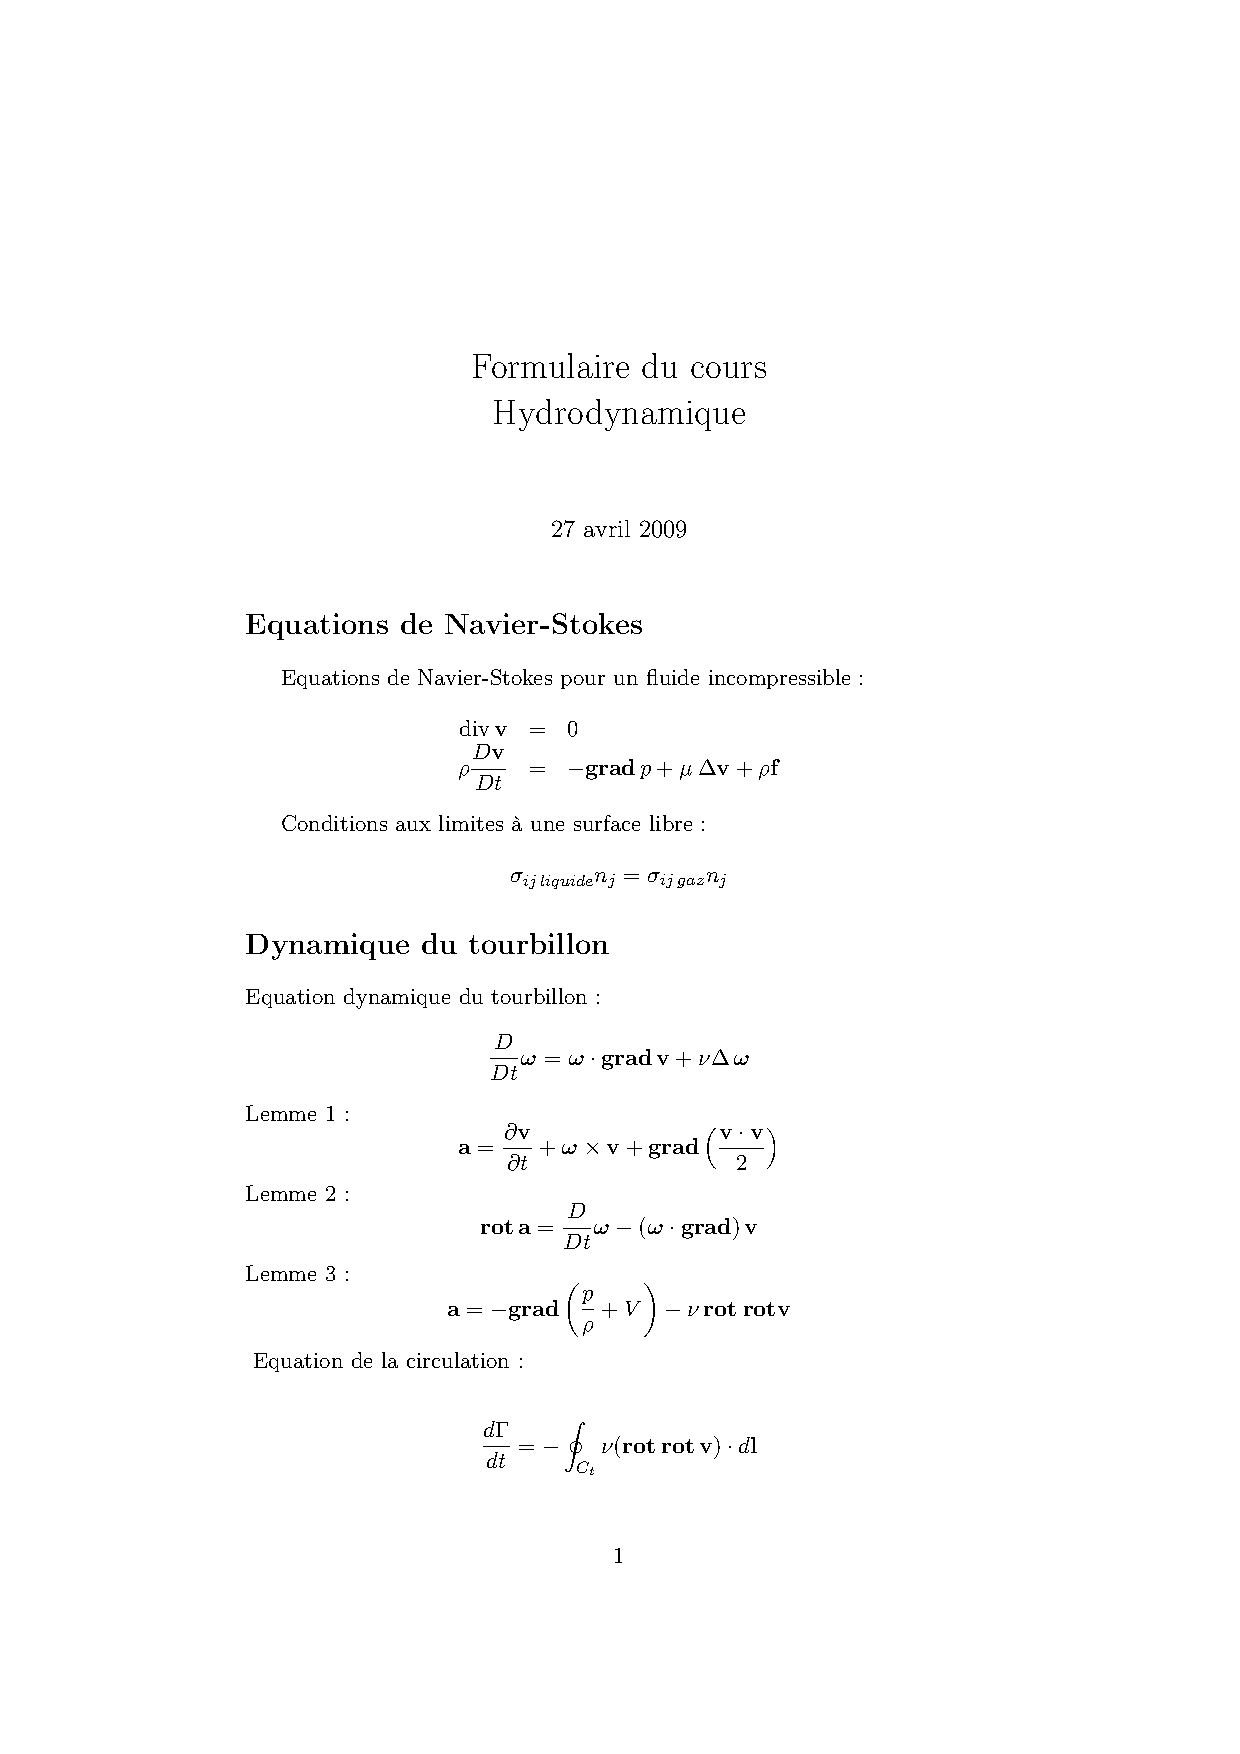
\includepdf[pages={1-},nup={2x2}, trim = 2cm 2cm 2cm 2cm, scale = 1.05]{pdf/_formulairehydro.pdf}
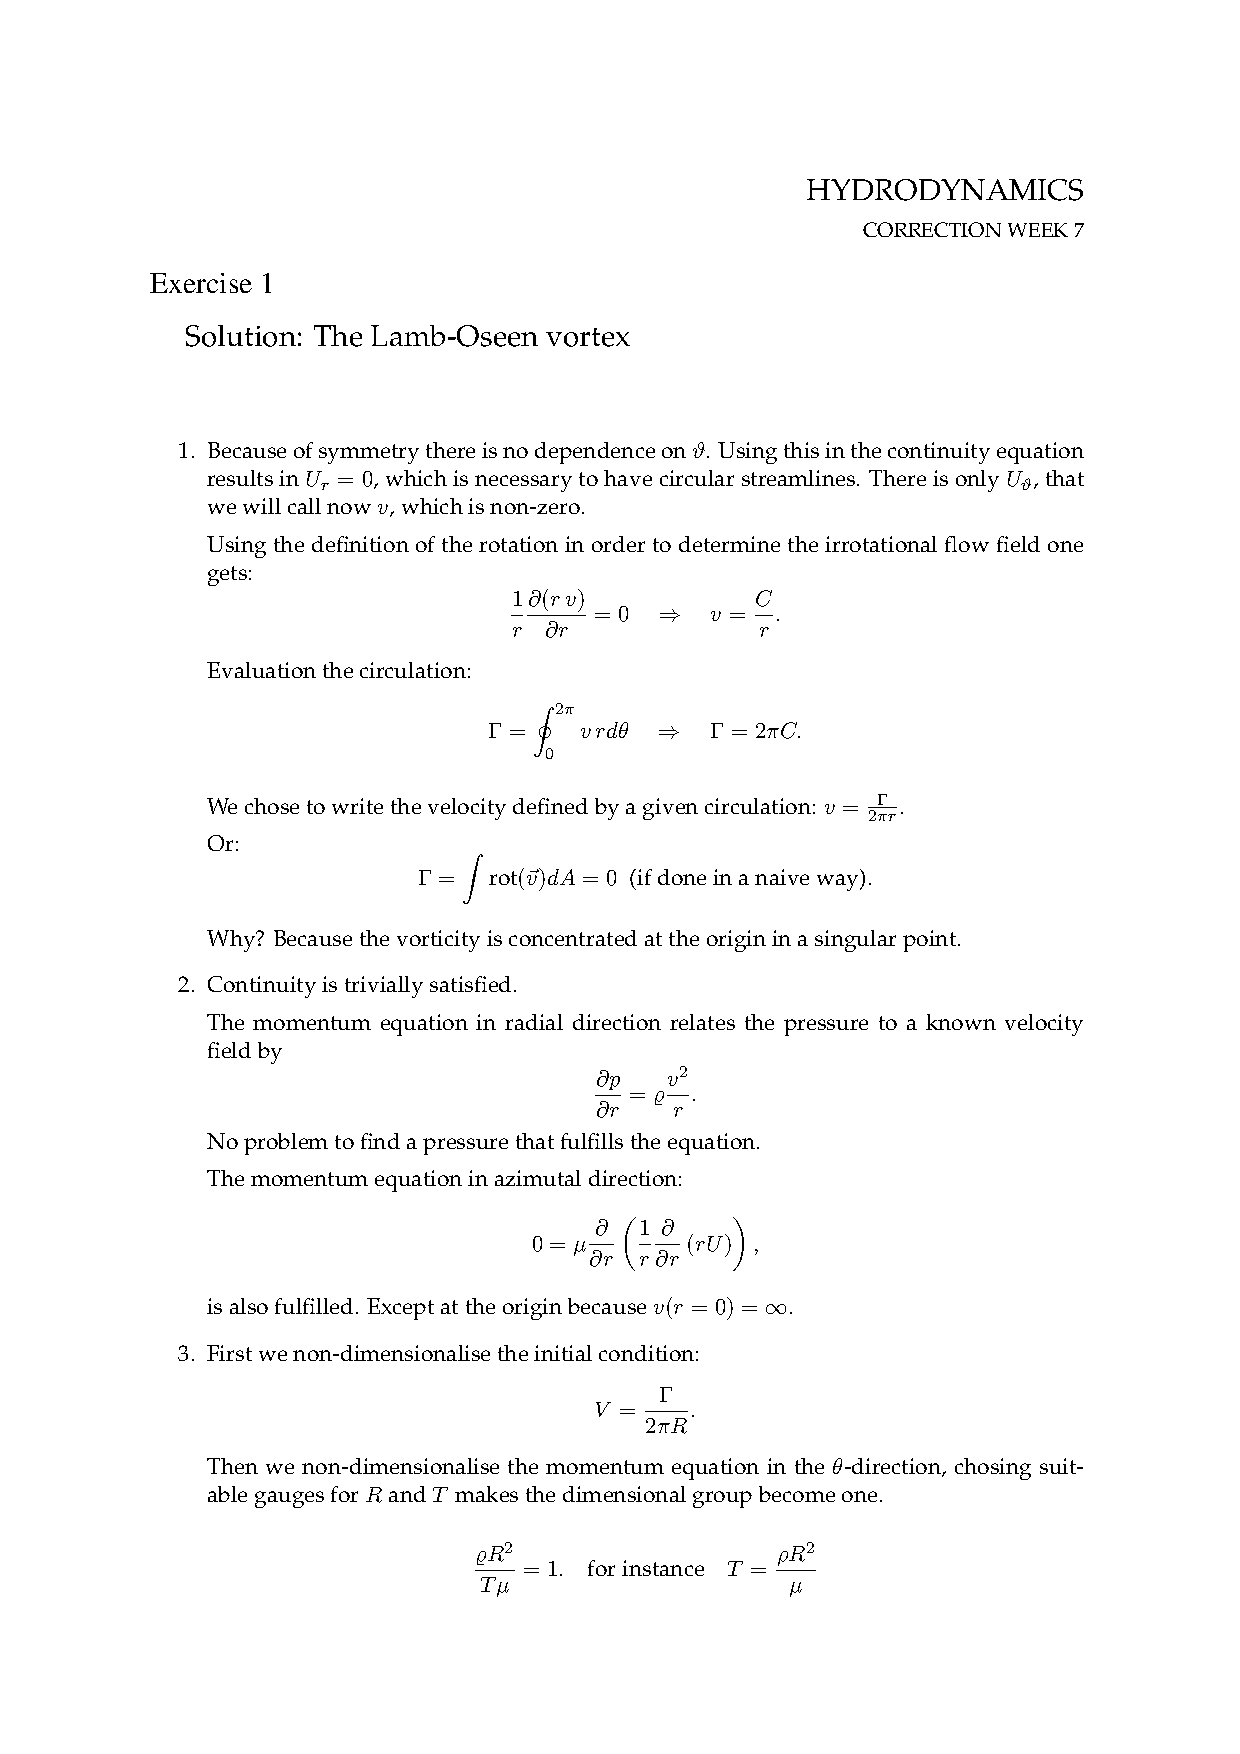
\includepdf[pages={1-},nup={2x2}]{pdf/_hydro-corr-07.pdf}

\end{document}
